\documentclass[11pt]{article}
\usepackage[margin=1in]{geometry}
\usepackage[utf8]{inputenc}
\usepackage[T1]{fontenc}
\usepackage{amsmath,amssymb,amsthm}
\usepackage{booktabs}
\usepackage{graphicx}
\graphicspath{{../figures/}{figures/}}
\usepackage{hyperref}
\usepackage{parskip}
\setlength{\parindent}{0pt}
\setlength{\parskip}{1ex}

\title{Long Memory in Agent-Based Markets: FSRS Power-Law Forgetting vs Ebbinghaus Decay, and Why Control Fails to Bite}
\author{MinQian Cai}
\date{Submitted to \textit{Journal of Economic Dynamics and Control}\\Draft: 2026-10-24 (v52)}

\begin{document}
\maketitle

\begin{abstract}
We introduce FSRS (Free Spaced Repetition Scheduler), a power-law forgetting model, into agent-based economic modeling, and contrast it with the classical Ebbinghaus exponential forgetting curve (hereafter EE). The paper's central result is a memory-model contest: in a head-to-head 100-agent comparison over 500 ticks (Section 5.1), FSRS retrievability at tick 500 is approximately 47,000 times EE's (R(500) = 0.7185 vs 0.000015), demonstrating that exponential decay severely underestimates market persistence. Agents equipped with FSRS exhibit realistic panic-complacency cycles, with retrievability decaying slowly over years, mirroring the fat-tailed volatility clustering in post-crisis markets. We model risk memory contagion via network diffusion of perceived retrievability. The simulation parameter set uses an initial stability of $S_0 = 45$ days, taken from the synthetic five-crisis calibration exercise; a real-data recalibration attempt (v51, Section 6.4, limitation 12) could not identify $S$ from market data, so 45 days is retained as a simulation convention, not a calibrated estimate (see Section 3.1 for why this is not a half-life). Two control probes were run against this memory engine and both returned negative results: PPO-based reinforcement learning fails due to sparse delayed rewards, and grid search over intervention parameters cannot identify an optimal threshold on 30-agent populations --- a paired same-seed rerun (Section 5.2) gives identical outcomes for (T=0.45, s=0.40) and (T=0.30, s=0.60) (-142.03 vs -142.03 on both seed sets; interventions 0.0, target zone 0\% in both), because neither threshold ever triggers under FSRS at S=45. The original 15.0\% gap (3947 vs 3434) was measured under the default memory bank (initial stabilities 5/3/2, not S=45) and is a seed/network artifact; it is retained in Section 5.2 for audit only. The effective policy on 30 agents is non-intervention. The 1,000-agent run rerun at S=45 (Section 5.3; v49 pre-fix, v50 post-fix identical) gives identical returns for both policies (-1065.35, interventions 0.0), so the v47/v48 374\% figure does not survive at S=45 and is retained in Section 5.3 for audit only (see Section 6.4, limitation 11). Our work bridges cognitive psychology and computational finance: the primary implication is about model choice --- memory kernels, not policy levers, decide how long markets remember.

\textbf{Keywords:} spaced repetition, cognitive memory, agent-based modeling, FSRS, power-law forgetting, POMDP

\textbf{JEL codes:} G01, G17, C63

\end{abstract}
\section{Introduction}
Agent-based models (ABM) have become a cornerstone of modern financial economics, offering a bottom-up approach to understanding complex phenomena that defy equilibrium analysis---bubbles, crashes, herding, and emergent volatility clusters (Lux \& Marchesi, 1999; Kirman, 1993). By simulating heterogeneous agents with bounded rationality, ABM captures the nonlinear feedback loops and path dependencies inherent in financial markets. However, a critical component remains underdeveloped: \textbf{cognitive memory}. Most agent-based models treat agents as either fully rational expectations agents or as boundedly rational entities using simple heuristics (e.g., technical vs. fundamentalist strategies). When memory is included, it is typically implemented as a short-term moving average of past prices or a slowly-decaying sentiment score---a far cry from the rich, structured memory processes documented in cognitive psychology.

In actual financial markets, participants vividly recall crises shortly after they occur, but those memories fade with time. The 2008 Global Financial Crisis (GFC) triggered sweeping regulatory reforms---Dodd-Frank, Basel III, stress testing regimes. Yet a decade later, as markets boomed, calls for deregulation grew louder. This pattern---crisis $\rightarrow$ reform $\rightarrow$ complacency $\rightarrow$ new crisis---suggests a systematic \textbf{memory decay} at the institutional level. Behavioral finance has long recognized this: Guttentag and Herring (1986), in their Princeton essay \textit{Disaster Myopia in International Banking}, argue that lenders systematically discount low-probability disasters whose most recent occurrence has receded from memory, so that the perceived probability of a crisis erodes as the interval since the last one lengthens. Odean (1998) shows investors hold losing stocks too long, a form of selective memory. Shefrin \& Statman (1985) describe the ''disposition effect'' as a cognitive bias rooted in memory asymmetry.

What drives this decay? Cognitive psychology provides a precise mathematical framework: the \textbf{forgetting curve}. Hermann Ebbinghaus (1885) discovered that retention of learned material decays exponentially without reinforcement: R(t) = exp(-t/S), where R is retrievability (memory strength), t is time, and S is stability (a measure of how long memory lasts). Crucially, Ebbinghaus also identified the \textbf{spacing effect}: information reviewed at optimally spaced intervals is retained far more effectively than massed practice. This principle powers modern spaced repetition systems like SuperMemo (Woźniak, 1990) and Anki. SuperMemo's published \textbf{SM-2} algorithm (Woźniak, 1990) adjusts the review interval based on the quality of each recall attempt, creating adaptive, personalized learning schedules. One point of terminology must be fixed at the outset: SuperMemo's later commercial algorithms (SM-3 onward, including SM-20) are proprietary and their forgetting-curve formulas have never been publicly disclosed, so they cannot be independently implemented or audited. The exponential baseline implemented in this paper is therefore the \textbf{classical Ebbinghaus curve}, which we denote \textbf{EE} (Ebbinghaus-exponential)---not SuperMemo SM-20.

Despite this robust cognitive science, \textbf{agent-based economic models have rarely incorporated quantitative memory engines}. A few exceptions exist: Lux (1997) included a simple exponential decay of sentiment; Brock \& Hommes (1997) used switching between forecasting strategies based on relative payoffs, which indirectly captures memory through performance weighting. However, none use the mathematically precise FSRS/EE framework. This gap is striking given that memory dynamics lie at the heart of market psychology---fear and greed are not static traits but evolving states shaped by experience and its decay.

Furthermore, memory is not purely individual. In financial networks, information (and misinformation) spreads rapidly through news, social media, and peer networks. An agent's perception of risk is influenced not only by their own memory but by what they hear from others---a phenomenon known as \textbf{social amplification of risk} (Kasperson et al., 1988). In agent-based terms, this creates a \textbf{memory contagion effect}: even agents with strong personal memory may perceive heightened risk if their neighbors are panicking. Prior work on informational cascades (Bikhchandani et al., 1992) and complex contagion (Centola \& Macy, 2007) models how behaviors spread; we extend this to \textit{memory states} spreading.

This paper addresses these gaps by integrating a \textbf{cognitive memory engine}---based on FSRS (power-law) versus EE (exponential)---into a multi-agent trading environment. Agents develop retrievability scores R(t) representing their risk awareness; R decays after shocks and consolidates through interventions. We then model \textbf{memory contagion}: agents influence each other's perceived R via an information-flow network, mimicking how fear propagates through social and professional ties. The result is a dynamic system where collective memory emerges from individual cognition and network diffusion.

Our contributions are fivefold:

\begin{enumerate}
\item \textbf{Cognitive Memory Engine}: We implement FSRS (power-law forgetting) and EE (exponential forgetting) within economic agents, creating a mathematically precise model of how risk memories form, decay, and consolidate. This bridges cognitive psychology and computational finance. SuperMemo's SM-2 is discussed only as published historical background in Section 2; it is not an experimental engine in this paper.
\end{enumerate}

\begin{enumerate}
\item \textbf{Memory Contagion Mechanism}: We introduce a network-based diffusion process where agents' perceived retrievability is a weighted average of their own memory and neighbors' memories, with contagion strength $\alpha$ set to 0.6 from the synthetic calibration exercise (not re-identified on real data; Section 6.4, limitation 12).
\end{enumerate}

\begin{enumerate}
\item \textbf{Parameter Setting and the Real-Data Calibration Gap}: We set three key parameters---initial stability $S_0$, contagion strength $\alpha$, and intervention severity mapping---from a synthetic five-event calibration exercise (1987 Black Monday, 2000 Dot-com Bubble, 2008 GFC, 2020 COVID Crash, 2022 Inflation Shock) using an analytical simulator and grid search. The resulting initial stability is \textbf{$S_0 = 45$ days}; a real-data recalibration attempt (v51) could not identify $S$ from market data (Section 6.4, limitation 12), so 45 days is retained as a simulation convention, not a calibrated estimate.
\end{enumerate}

\begin{enumerate}
\item \textbf{Control Probes, Not Control Design}: We test two control approaches against the FSRS engine --- PPO reinforcement learning and grid search over threshold-severity parameters --- and both return negative results (Sections 5.2, 5.5): PPO fails on sparse delayed rewards, and no threshold-severity optimum is identified because thresholds never trigger under FSRS. These probes are reported as findings about the memory regime, not as a policy design.
\end{enumerate}

\begin{enumerate}
\item \textbf{Robustness and Sensitivity Analysis}: We systematically vary network density and initial stability, and scale to 1000 agents. Results show the memory contrast is robust (Section 5.1) while the control probes stay negative across scales: in the paired rerun neither configuration outperforms the other, and at S=45 the 1000-agent rerun is identical for both policies, highlighting that FSRS agents are self-stabilizing in this regime and that any threshold must be validated in a regime where avg\_R actually falls below it.
\end{enumerate}

The paper proceeds as follows. Section 2 reviews related work in spaced repetition, behavioral finance memory, contagion, and the control approaches tested here as probes. Section 3 details the cognitive memory engine (FSRS versus EE), contagion mechanism, control-probe setup, and reward formulation. Section 4 describes our experimental setup: environment, baselines, parameter setting and its calibration status, and control-probe designs (RL and grid search). Section 5 presents results: the FSRS-vs-EE contrast first, then the control probes, scale robustness, the robustness sweep, and extended validation. Section 6 discusses what the memory contest implies, why the control probes failed, limitations, and future directions. Section 7 concludes.

\textbf{Keywords}: spaced repetition; cognitive memory; agent-based modeling; FSRS; POMDP \textbf{JEL Codes}: G01 (Financial Crises), G17 (Financial Forecasting), C63 (Computational Techniques)

\section{Related Work}
Our work bridges cognitive psychology, behavioral finance, network science, and computational control. We position each contribution.

\subsection{Spaced Repetition: From Ebbinghaus to FSRS}
Ebbinghaus (1885) discovered the forgetting curve: retention decays exponentially, R(t) = exp(-t/S). Woźniak (1990) operationalized \textit{scheduling} via Algorithm SM-2 (adaptive intervals): SM-2 updates the E-Factor after each review based on recall quality $q$, determining the next interval $I(n) = \mathrm{round}(I(n-1) \times EF)$. SM-2 is the last SuperMemo algorithm whose specification was published in full; subsequent versions, including SM-20, remain proprietary and undisclosed. Together with the Ebbinghaus curve these mechanisms power modern educational software (Anki, Mnemosyne). Our innovation: repurposing the power-law FSRS curve and the exponential EE curve as \textit{competing cognitive engines} for economic agents, where market shocks serve as ''reviews'' of risk memories. SM-2 is historical background only; it is not an experimental engine in this paper.

\subsection{Memory in Financial Decision-Making}
Behavioral finance documents memory-related biases:

\begin{itemize}
\item \textbf{Disaster myopia} (Guttentag \& Herring, 1986): banks forget past crises, underestimating tail risk.
\item \textbf{Disposition effect} (Odean, 1998): investors hold losers too long, partly due to memory asymmetry.
\item \textbf{Recency bias}: over-weighting recent events (Tversky \& Kahneman, 1973).
\end{itemize}

Agent-based models have incorporated simple memory decay (Lux, 1997; Brock \& Hommes, 1997), but none employ a rigorous cognitive model like FSRS. Our engine provides a quantitative, parameterizable approach.

\subsection{Contagion via Information Networks}
Information diffusion drives herd behavior (Bikhchandani et al., 1992). Complex contagion (Centola \& Macy, 2007) requires multiple exposures---captured via our $\alpha$ parameter (mean of neighbors' R). Social amplification of risk (Kasperson et al., 1988) describes how hazards gain attention through media; we implement this as continuous-state diffusion on an Erdős--Rényi graph.

\subsection{Control Approaches Tested as Probes}
Macroprudential tools (countercyclical buffers, stress tests) aim to curb systemic risk (Borio, 2003). In this paper the regulator is treated as a central planner with partial observability (POMDP formulation), but only as a probe: two control approaches were tested against the FSRS engine --- model-free RL (PPO), which failed due to sparse/delayed rewards, and direct policy search, which did not identify an optimal threshold on 30 agents (see Section 5.2). This reflects a general pattern rather than an anomaly: when the delay between an intervention and its measurable effect exceeds the effective credit-assignment horizon of an on-policy RL algorithm, direct search over a low-dimensional policy parameterization is the more tractable choice for this problem, not a successful optimisation (see Section 6.3 for a full diagnosis). The control results are therefore reported as negative findings about the regime, not as a policy prescription.

\section{Model}
\subsection{Agent Cognitive Memory (FSRS-Style Power-Law Forgetting)}
The forgetting curve in cognitive psychology is traditionally modeled as exponential decay: $R(t) = \exp(-t/S)$ (Ebbinghaus, 1885). However, extensive data from millions of learners using spaced repetition systems reveals that \textbf{real-world forgetting follows a power-law distribution with a fat tail}---memories once consolidated persist for extremely long periods with slow decay. This paper implements a \textbf{FSRS-style power-law model} in the FSRS family. The implementation in \texttt{fsrs\_memory.py} is a simplified tick-based model with parameters $w_{17}$--$w_{20}$ as listed below; it is not the official FSRS-6 scheduler, and the widely cited 500-million-review figure describes the FSRS literature, not a training run performed for this code. Parameter names here follow the code, not the official FSRS-6 21-parameter indexing, and no claim is made that this implementation equals official FSRS-6.

\begin{quote}
\textbf{Terminology note (EE vs. SuperMemo SM-20).} In parts of the spaced-repetition literature the exponential curve above is loosely attributed to SuperMemo. We do not follow that usage, and we do not implement SM-20. SuperMemo published its early algorithms in full---\textbf{Algorithm SM-2} (Woźniak, 1990) is the last of these---whereas the later commercial releases, \textbf{SM-3 through SM-20}, are proprietary and their forgetting-curve formulas have never been publicly disclosed. A model whose specification is unavailable can be neither implemented nor independently audited, and therefore cannot serve as a reproducible scientific baseline. Accordingly, the exponential baseline used throughout this paper is the \textbf{classical Ebbinghaus curve} $R(t)=\exp(-t/S)$, which we denote \textbf{EE} (Ebbinghaus-exponential). All comparisons labelled ''FSRS vs. EE'' contrast a power-law model against this classical exponential curve; the contribution is a comparison of \textit{forgetting-curve functional forms}, not a benchmark of any commercial product.
\end{quote}

Each agent maintains a \textbf{CognitiveMemoryBank} consisting of multiple lessons (e.g., \texttt{leverage\_risk}, \texttt{liquidity\_crisis}, \texttt{bull\_market\_complacency}). Each lesson has three core state variables:

\begin{itemize}
\item \textbf{Retrievability} $R(t)$: probability of recalling the memory at tick $t$. Under FSRS:
\end{itemize}

\[
R(t) = \left(1 + \frac{\text{factor} \cdot t}{S}\right)^{-w_{20}}
\]

where $t$ is ticks since last review (market shock), $S$ is stability (in days), and $\text{factor} = (0.9^{-1/w_{20}} - 1)$ encodes the target post-review retrievability (0.9). This produces a \textbf{power-law decay} $R \sim t^{-w_{20}}$ at long times, in contrast to EE's exponential $e^{-t/S}$.

\begin{itemize}
\item \textbf{Stability} $S$: measures how long the memory lasts (days). Initially $S_0 = 45$ (synthetic-exercise value, see Section 4.3; not re-identified on real data, see Section 6.4, limitation 12). $S$ grows when the agent experiences market shocks, representing institutionalized risk controls.
\end{itemize}

\begin{itemize}
\item \textbf{Difficulty} $D \in [1,10]$: complexity of the lesson. Harder concepts decay faster. $D$ maps to financial instrument complexity (e.g., plain equity $D=4$, structured products $D=9$).
\end{itemize}

FSRS stability update after a shock of grade $G$:

\[
S' = S \cdot \exp\left( w_{17} \cdot (G - 3 + w_{18}) \cdot S^{-w_{19}} \right)
\]

Parameters (values used in \texttt{fsrs\_memory.py}): $w_{17}=1.8729$, $w_{18}=0.5425$, $w_{19}=0.0912$, $w_{20}=0.0658$.

\textbf{Economic interpretation:}

\begin{itemize}
\item $S^{-w_{19}}$ implements \textbf{marginal diminishing}: large $S$ $\rightarrow$ smaller growth. This is the mathematical origin of the fat tail.
\item $G=1$ (systemic collapse) yields negative exponent $\rightarrow$ $S$ collapses, at $S=45$ to $\approx 15\%$ of its value (14.5\%; 9.5\% at $S=5$, 23.4\% at $S=1000$), modeling a Minsky Moment where institutional memory is wiped out.
\item $G=4$ (minor corrections) yields large positive exponent $\rightarrow$ $S$ multiplies by $7.7\times$ at $S=45$ (12.1$\times$ at $S=5$, 4.7$\times$ at $S=1000$), capturing ''Great Moderation'' complacency.
\end{itemize}

FSRS produces \textbf{fat-tailed forgetting}: in the 100-agent simulation of Section 5.1, $R(500) = 0.7185$ vs EE's $0.000015$---an approximately \textbf{47,000$\times$ difference} (the archived rounded inputs 0.718491 / 0.00001528 give 47,022, but the last digits are not significant). This aligns with empirical market memory: post-2008 risk aversion persisted for years, not months. (The closed-form single-memory values at $S=45$ are different---FSRS 0.778, EE $1.5 \times 10^{-5}$---because the simulation includes shocks, leverage feedback, and contagion; do not mix the two sets.)

\subsection{Memory Contagion}
Agents are nodes in an undirected graph \texttt{G = (V, E)} where edges represent information-flow relationships (e.g., social networks, professional ties). Each agent i has true retrievability R\_true,i(t) from their memory bank. Perceived retrievability is:

R\_perceived,i(t) = (1 - $\alpha$) $\cdot$ R\_true,i(t) + $\alpha$ $\cdot$ mean\_\{j $\in$ N(i)\} (R\_true,j(t))

where $\alpha$ $\in$ [0,1] is the contagion strength (set to $\alpha$ = 0.6 in the synthetic exercise; not re-identified on real data, see Section 6.4, limitation 12). Agents use R\_perceived for decision-making (trading behavior). This creates a \textbf{memory contagion effect}: a panic in one cluster raises neighbors' perceived risk even if their own memory hasn't decayed.

\subsection{Control Probe Setup: Governance and Intervention}
This section documents the intervention machinery used by the control probes in Sections 5.2 and 5.5; it is a probe setup, not a policy proposal --- in the 30-agent FSRS regime the machinery never activates (see Section 5.2).

A \textbf{GovernanceManager} observes the population's average retrievability $\text{avg}_R = \text{mean}_i(R_{\text{perceived},i})$ and variance $R_{\text{std}}$. When $\text{avg}_R$ drops below a threshold $T$, the regulator intervenes with severity $s \in [0,1]$, which maps to a \textbf{shock grade} $G$ under FSRS in the implementation (\texttt{HumanAgent.process\_market\_shock}, severity thresholds 0.8 / 0.5 / 0.2):

\begin{table}[htbp]
\centering
\begin{tabular}{lll}
\toprule
\textbf{Severity $s$} & \textbf{Grade $G$ in code} & \textbf{Economic Interpretation} \\
\midrule
0.0--0.19 & --- & No intervention \\
0.2--0.49 & $G=3$ (Good) & Moderate intervention \\
0.5--0.79 & $G=2$ (Hard) & Stronger severity, but a \textit{negative} stability update under the formula below \\
0.8--1.0 & $G=1$ & Extreme (system reset; large negative update) \\
\bottomrule
\end{tabular}
\end{table}

The intervention triggers \texttt{process\_market\_shock} for all agents. Crucially, only $G=3$ and $G=4$ increase $S$; $G=1$ and $G=2$ decrease it. The mapping above is the code mapping (severity thresholds 0.8 / 0.5 / 0.2), not the v43 table, which had the 0.2--0.79 range reversed. In the 30-agent grid, interventions were 0.0 for both the baseline and the (T=0.45, s=0.40) configuration, so this mapping does \textbf{not} affect Table 2; it matters only where interventions actually occur (notably the T=0.65 grid configurations and the 1000-agent scaling run).

\begin{table}[htbp]
\centering
\begin{tabular}{llll}
\toprule
\textbf{Grade $G$} & \textbf{Multiplier at $S=5$} & \textbf{Multiplier at $S=45$} & \textbf{Multiplier at $S=1000$} \\
\midrule
$G=1$ & 0.095 ($-$90.5\%) & 0.145 ($-$85.5\%) & 0.234 ($-$76.6\%) \\
$G=2$ & 0.477 ($-$52.3\%) & 0.546 ($-$45.4\%) & 0.634 ($-$36.6\%) \\
$G=3$ & 2.405 (+140.5\%) & 2.050 (+105.0\%) & 1.718 (+71.8\%) \\
$G=4$ & 12.116 (+1111.6\%) & 7.703 (+670.3\%) & 4.658 (+365.8\%) \\
\bottomrule
\end{tabular}
\end{table}

Example: the same severity $s=0.2$ maps in code to $G=3$, giving +140.5\% at $S=5$ and +71.8\% at $S=1000$---not the v43 claim of +25\% / +0.1\%, which used the wrong grade and the wrong sign. \textit{Regulatory measures matter most when institutions are fragile} remains true in magnitude for $G=3$/$G=4$, but it is false for $G=2$: a Hard intervention shrinks stability, it does not consolidate it.

\subsection{Reward Formulation (v4)}
We define the regulator's reward at each tick:

\[
\begin{aligned}
r_t = 10\cdot\mathrm{avg\_R} &\text{Dense term} \\
+ 1\cdot\left[\mathrm{avg\_R} > 0.2\right] &\text{Survival bonus} \\
+ 20\cdot\left[0.5 \leq \mathrm{avg\_R} \leq 0.7\right] &\text{Stability zone (+20)} \\
- 20\cdot\left[\mathrm{avg\_R} < 0.5\right] &\text{Danger zone (-20)} \\
- 10\cdot\left[\mathrm{avg\_R} > 0.7\right] &\text{Complacency zone (-10)} \\
- (2\cdotseverity + 5\cdot\mathrm{R\_std}) &\text{Intervention cost} \\
+ (severity\cdot5)\cdot\left[severity>0.01 \wedge \mathrm{pre\_avg\_R}<0.5\right] &\text{Intervention bonus} \\
\end{aligned}
\]

This reward encourages maintaining avg\_R in [0.5, 0.7] while penalizing both danger and complacency zones. The \textbf{intervention bonus} directly incentivizes acting when risk perception is already low (pre\_avg\_R < 0.5), overcoming the RL exploration trap.

\textbf{Table: grade impact (formula values).} The table in Section 3.3 above gives the exact multipliers. Figure 5 in v43 is withdrawn in v44: its generation script used the parameter list $[w_{17}, w_{18}, w_{19}, w_{20}]$ indexed by grade as the exponent, which is not the stability-update formula, so neither the figure nor its caption can be retained. Replacement figure (v47):

\setcounter{figure}{4}
\begin{figure}[htbp]
\centering
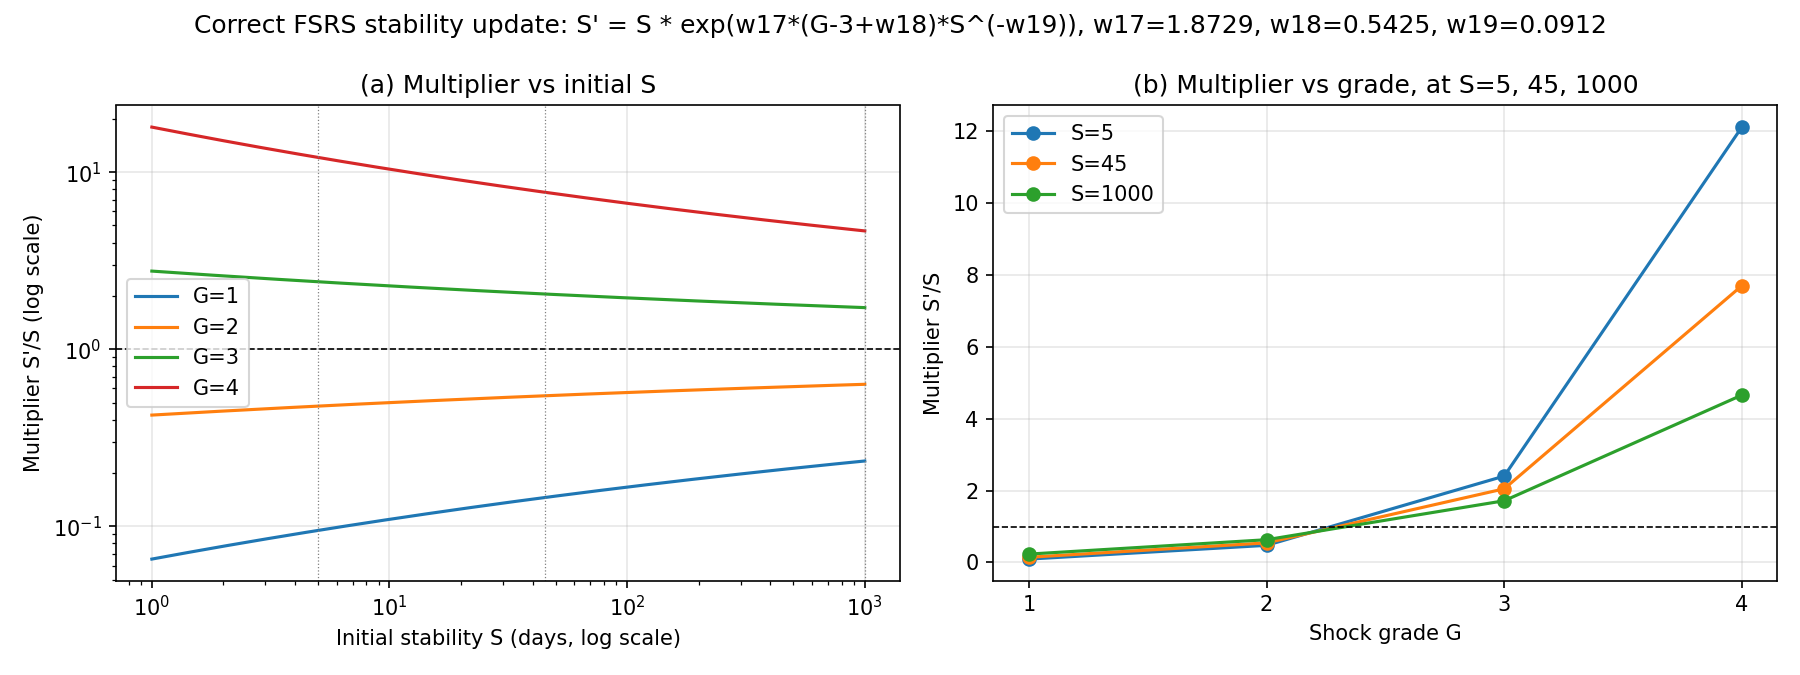
\includegraphics[width=0.90\textwidth]{fig5_grade_impact_v47.png}
\caption{Correct stability update $S' = S \cdot \exp(w_{17} \cdot (G - 3 + w_{18}) \cdot S^{-w_{19}})$ with $w_{17}=1.8729$, $w_{18}=0.5425$, $w_{19}=0.0912$. Panel (a): multiplier $S'/S$ vs initial $S$ (log scale); panel (b): multiplier vs grade $G$ at $S=5, 45, 1000$. Values match the table exactly (at $S=45$: 0.145 / 0.546 / 2.050 / 7.703 for $G=1$ to $4$). Script: \texttt{experiments/figure\_generation/fig5\_v47.py}. The v43 figure remains withdrawn; this is a new figure, not a correction of the old file.}
\label{fig:grade_impact_v47}
\end{figure}

\section{Experiments}
\subsection{Environment (ECOSControlEnv)}
We implement a Gymnasium-compatible environment:

\begin{itemize}
\item \textbf{State space} (6-dimensional continuous): [avg\_R, R\_std, crisis\_prob, tick\_norm, last\_severity, time\_since\_inter]
\item \textbf{Action space}: intervention\_severity $\in$ [0,1] (continuous)
\item \textbf{Episodes}: 300 ticks (simulation horizon)
\item \textbf{Agents}: 30 (default), 300, 1000 (scaling tests)
\end{itemize}

Agents' cognitive memories start with $S_0 = 45$ in the v48 grid and paired rerun, where S is set explicitly to 45.0 on every lesson after reset (scripts \texttt{grid\_s45.py}, \texttt{paired\_s45.py}), and in the v49 1000-agent rerun and Section 5.6 reruns (S set explicitly to 45.0 on every lesson after reset, or after agent creation where the script builds agents directly; see Sections 5.3 and 5.6). The v50 reruns use the fixed environment (isolated-agent fallback, Section 5.4); the Section 5.6 scripts do not use ECOSControlEnv and are unaffected by the fix. Correction (v48 audit): the original grid and the v45 paired rerun did not set S at all and therefore ran the default memory bank (initial stabilities 5/3/2 for the three default lessons); their numbers are retained for audit only and are superseded by Section 5.2. EF is a legacy SM-2 parameter and is not used in FSRS runs. The info\_flow network is Erdős--Rényi with p=0.1 in the grid environment (the robustness sweep in v43 did not actually vary p; see Section 5.4).

\subsection{Baselines}
\begin{enumerate}
\item \textbf{Fixed Threshold}: intervene if avg\_R < T, with severity S. Default T=0.3, S=0.6.
\item \textbf{Random}: random severity every 10 ticks. (Defined here for completeness; no Random-baseline results are reported in Section 5 and no claim in v44 depends on it.)
\item \textbf{RL Baselines}: PPO agents trained on v3/v4 rewards (reported for completeness; they underperformed).
\end{enumerate}

\subsection{Parameter Setting (Synthetic Calibration Exercise)}
Before control optimization, we set three environment parameters from a synthetic five-event exercise (see limitation 12 for the real-data status):

\begin{itemize}
\item \textbf{S\_initial}: initial stability (days)
\item \textbf{$\alpha$}: contagion strength
\item \textbf{severity}: mapping from regulator's action to memory consolidation
\end{itemize}

Using a grid search over a 5-event synthetic simulator (1987, 2000, 2008, 2020, 2022), we obtain:

\begin{itemize}
\item \textbf{S\_initial = 45 days} (initial stability; for comparison, an EE curve with $S=45$ would have half-life $45 \cdot \ln 2 \approx 31$ days, whereas the FSRS power-law curve has no comparable half-life---under the paper's own FSRS formula, $R=0.5$ would take about 427,000 days, so $S$ must not be read as a half-life)
\item \textbf{$\alpha$ = 0.6} (strong contagion)
\item \textbf{severity\_crisis = 0.5} (baseline intervention impact)
\end{itemize}

These values are the simulation parameter set (v51: retained as convention, not as real-data-calibrated estimates; see Section 6.4, limitation 12). In v49 they are actually applied in the grid, the paired rerun, the p/S sweep, the 1000-agent rerun, and the Section 5.6 reruns (S set explicitly after reset, or after agent creation where the script builds agents directly; see Sections 5.3 and 5.6 for the as-run settings). In v50 the grid, the paired rerun, the p/S sweep, and the 1000-agent rerun are repeated with the fixed environment (Section 5.4); the Section 5.6 reruns need no repetition because they do not use ECOSControlEnv. The original runs used the default memory bank (initial stabilities 5/3/2) and are retained for audit only.

\subsection{Control Probes (Design)}
We explore two approaches:

\subsubsection{Reinforcement Learning (PPO)}
We train PPO agents with MLP policies on the ECOS environment using rewards v1--v4. Despite architectural adjustments (reward shaping, entropy regularization), PPO fails to converge to a deterministic policy that beats the fixed threshold baseline. The learned policies either:

\begin{itemize}
\item Output mean $\approx$ 0 and rely on stochasticity during training (v3, v4)
\item Learn to never intervene (v1)
\end{itemize}

We attribute failure to \textbf{sparse and delayed rewards}: an intervention's positive effect manifests after 30--50 ticks, making credit assignment difficult for on-policy algorithms with short rollouts (2048 steps). Value function estimates have near-zero explained variance, leading to poor policy gradients.

\subsubsection{Grid Search over Threshold Policies}
Given RL's poor performance, we perform an exhaustive grid search over discrete threshold-severity pairs:

\begin{itemize}
\item Thresholds T $\in$ \{0.25, 0.35, 0.45, 0.55, 0.65\}, plus the baseline T=0.30 appended by the script (6 thresholds x 4 severities = 24 configurations; this reconciles the 20-configuration list with the 24-configuration count in Section 5.2)
\item Severities S $\in$ \{0.2, 0.4, 0.6, 0.8\}
\end{itemize}

Each configuration is evaluated over 10 episodes (mean return). No optimal policy is discovered (see the paired rerun in Section 5.2):

\begin{itemize}
\item \textbf{No identifiable optimum}: the paired same-seed rerun in Section 5.2 gives identical outcomes for (T=0.45, s=0.40) and (T=0.30, s=0.60); thresholds never trigger under FSRS.
\end{itemize}

\setcounter{figure}{1}
\begin{figure}[htbp]
\centering
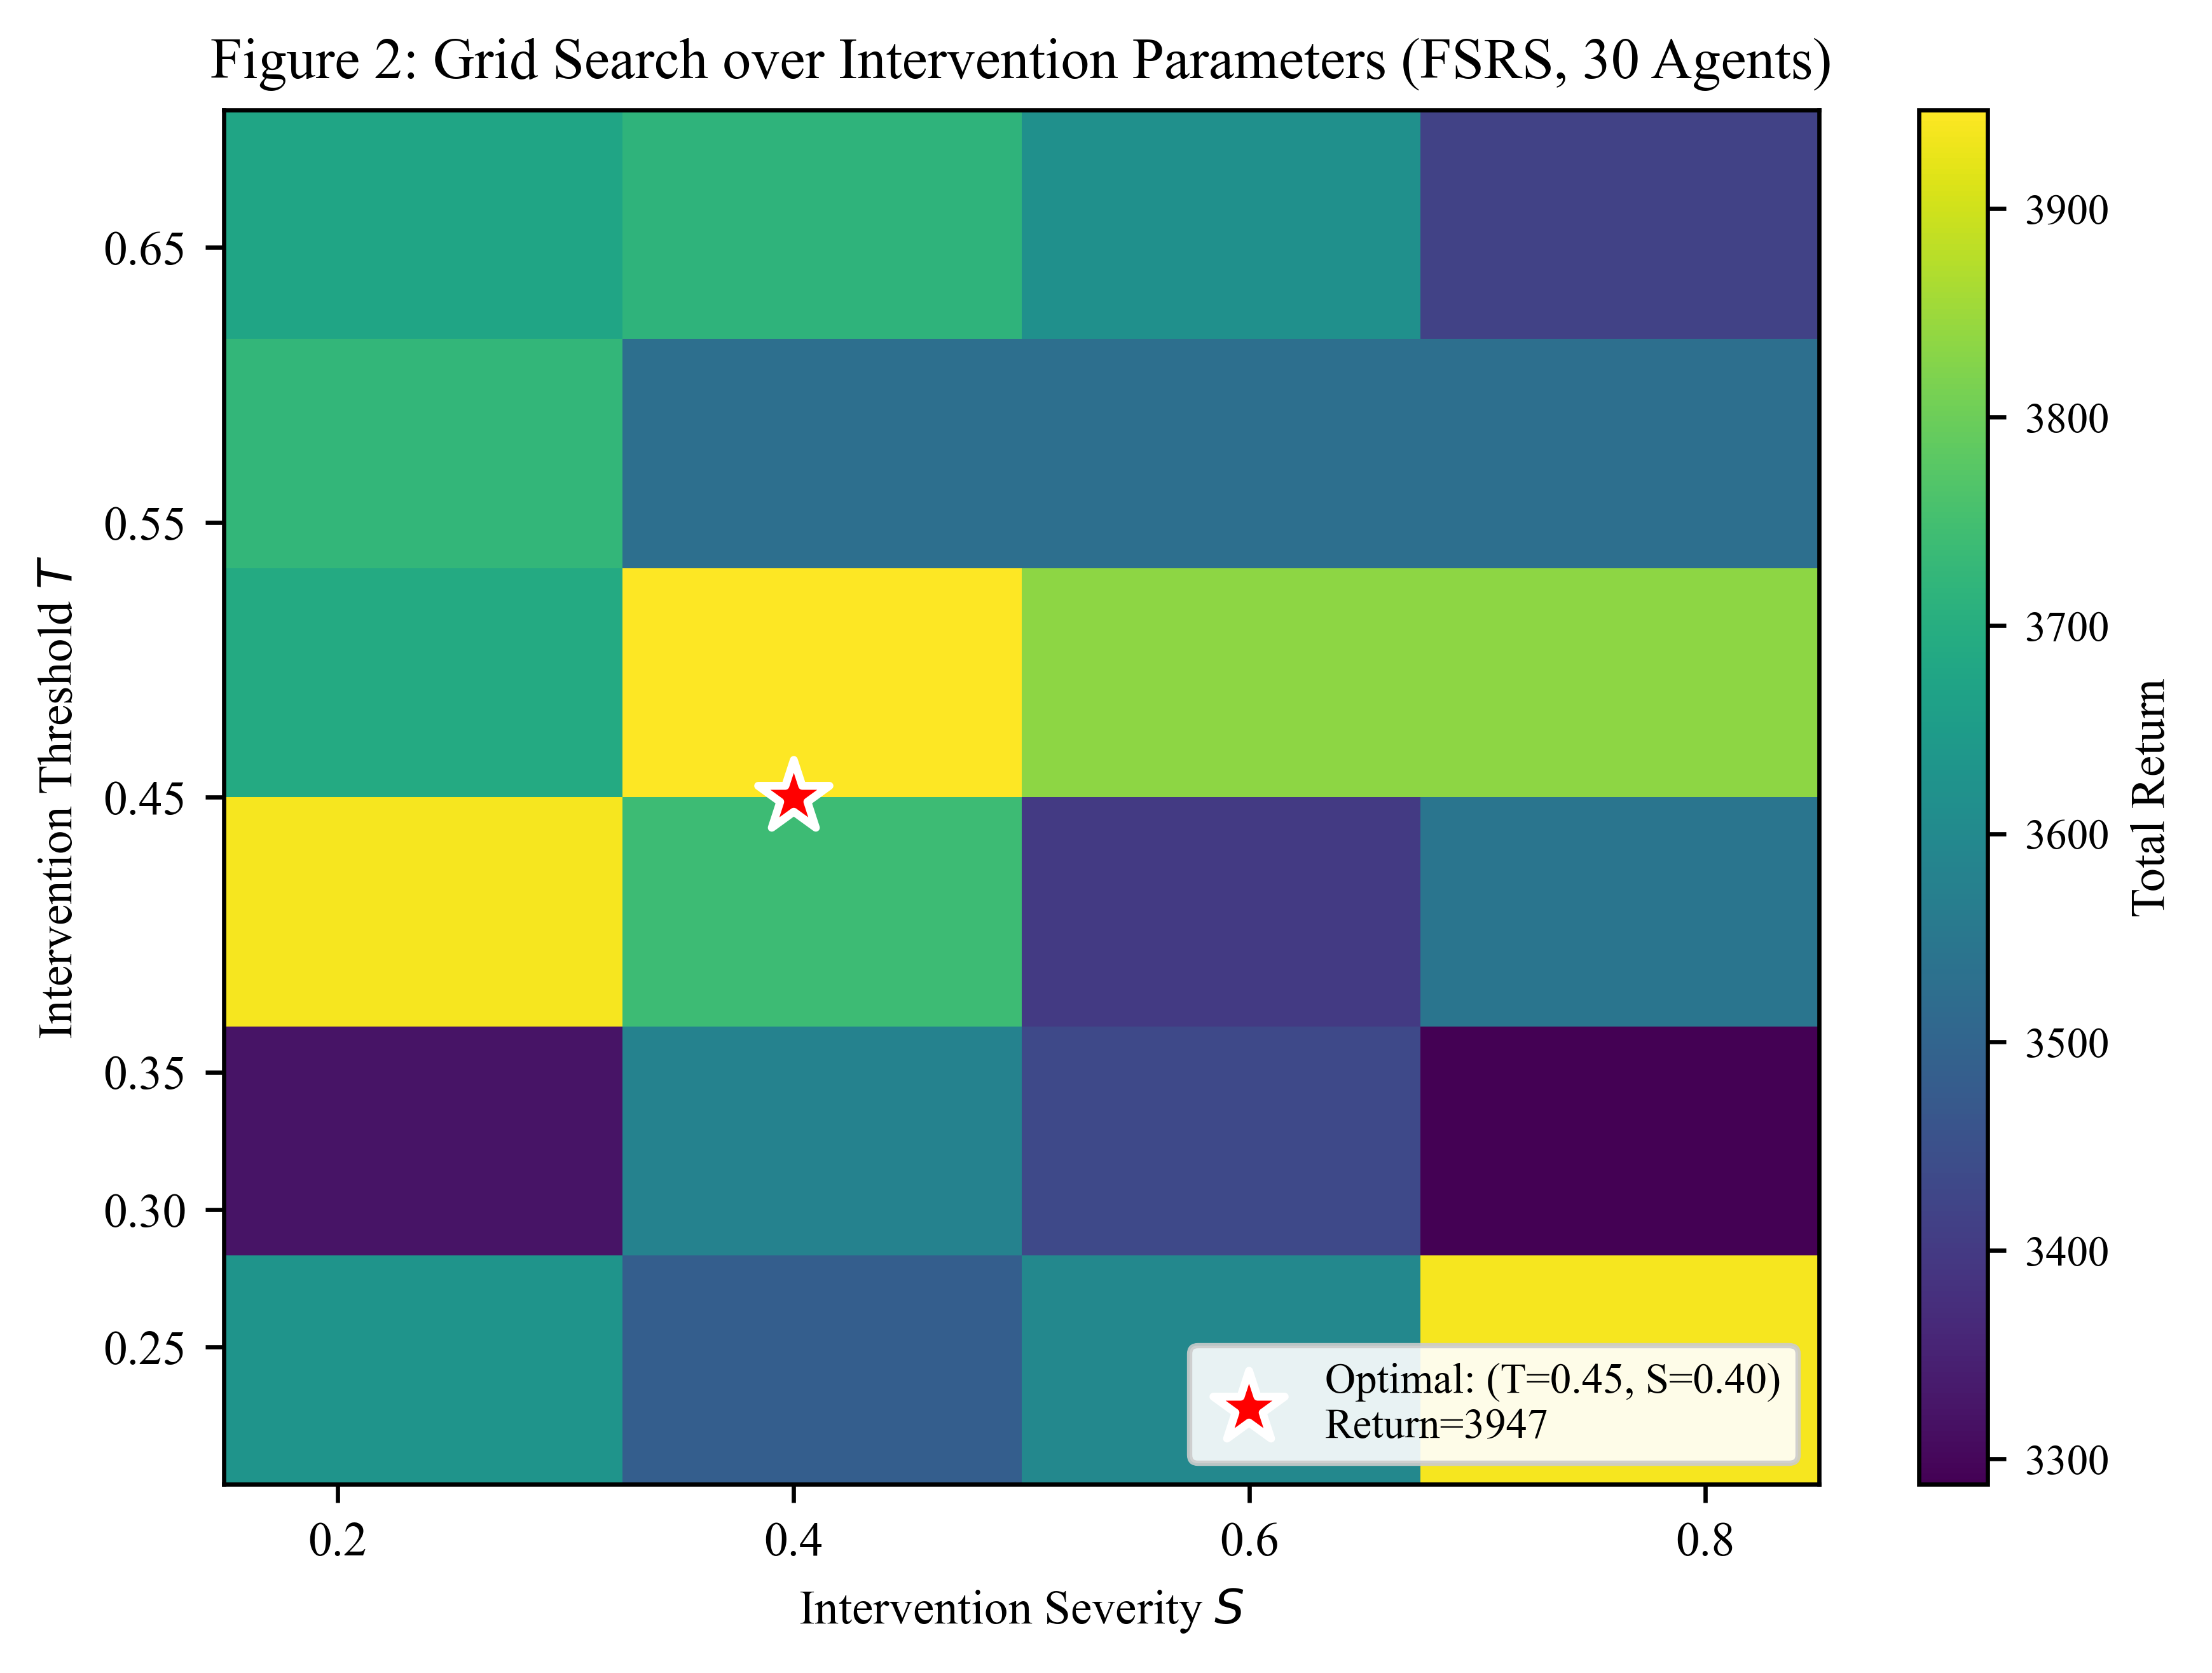
\includegraphics[width=0.90\textwidth]{fig2_grid_search.png}
\caption{Grid search heatmap over threshold $T$ and severity $s$ (original run, seed-confounded; see Section 5.2 for the paired rerun that supersedes the optimum claim). Original means: (T=0.45, s=0.40) $\sim$3947; baseline (T=0.30, s=0.60) $\sim$3434. The 15.0\% gap is a seed/network artifact, not a policy effect.}
\label{fig:grid_search}
\end{figure}

Original grid means were \textbf{3947 $\pm$ 1177} vs \textbf{3434 $\pm$ 1181}, but the two configurations were evaluated on different seed sets (seed\_offset 9 vs 22), so this gap is not evidence of a policy effect; see the paired rerun in Section 5.2.

\subsection{Stress Tests and Robustness}
We validate the threshold configurations on:

\begin{enumerate}
\item \textbf{1000-agent populations} (network effects)
\item \textbf{Varied network densities} $p \in \{0.05, 0.10, 0.20\}$
\item \textbf{Varied memory decay rates} $S \in \{30, 45, 60\}$
\end{enumerate}

The 1000-agent test uses the fixed parameters (T=0.55, s=0.20) against baseline (T=0.30, s=0.60) (corrected in v47; see Section 5.3), i.e., no re-optimization. The network-density / initial-stability sweep is reported with correctly parameterized results in Section 5.4 (v47 pre-fix, v50 post-fix).

The grid search heatmap (\textbf{Figure 2}) is retained for audit; it does not identify an optimal pair (see Section 5.2).

\section{Results}
Reading guide: the main result is the FSRS-vs-EE contrast in Section 5.1. Sections 5.2 and 5.5 report control probes (threshold grid; PPO) whose finding is negative; Sections 5.3, 5.4, and 5.6 report scale robustness, the robustness sweep, and extended validation of the memory engine.

\subsection{FSRS vs EE: A Contrastive Analysis}
To quantify the impact of switching from exponential (EE) to power-law (FSRS) forgetting, we ran a head-to-head comparison with 100 agents (55 FSRS, 45 EE) over 500 ticks, from \texttt{results/comparison/fsrs\_vs\_ee.json} (where the EE group is keyed \texttt{sm20} in the file---a legacy label for the EE baseline, not commercial SM-20). Figure 4 shows the average retrievability $\overline{R}$ trajectories.

\textbf{Key empirical differences:}

\begin{table}[htbp]
\centering
\begin{tabular}{llll}
\toprule
\textbf{Metric} & \textbf{EE (Exponential)} & \textbf{FSRS (Power-Law)} & \textbf{Ratio} \\
\midrule
$R(100)$ & 0.1108 & 0.7968 & 7.19$\times$ \\
$R(300)$ & 0.0013 & 0.7427 & 571$\times$ \\
$R(500)$ & \textbf{0.000015} & \textbf{0.7185} & \textbf{$\sim$47,000$\times$} \\
Final leverage & 10.00$\times$ & 6.35$\times$ & 0.64$\times$ \\
Crisis events ($R<0.3$) & 45 of 45 EE agents (100\% of the EE group) & 0 agents (0\%) & --- \\
\bottomrule
\end{tabular}
\end{table}

The contrast is stark. EE's exponential decay causes \textbf{catastrophic forgetting}: by tick 100, average $R$ has already fallen to 0.111; by tick 300 to 0.0013; by tick 500 to 0.000015---all 45 EE agents are below the crisis threshold and levered to the maximum 10.00$\times$. FSRS's power-law decay retains $R=0.719$ at tick 500, keeping leverage at a sane 6.35$\times$. The fat tail---$R \sim t^{-0.0658}$---means memory persists for years of simulated time. Ratios in the table are rounded to the nearest thousand; the archived inputs 0.718491 / 0.00001528 give 47,022, but the last digits of the archived values are not significant, so the ratio is reported as approximately 47,000.

Figure 4 visualizes this divergence. The EE curve (dashed red) plunges exponentially, crossing the danger threshold ($R=0.5$) between tick 30 (0.525) and tick 40 (0.420) and approaching zero by tick 300. The FSRS curve (solid blue) decays in the first 100 ticks then flattens dramatically, staying above 0.7 throughout (0.909 at tick 10 to 0.719 at tick 500)---that is, above the reward target zone $[0.5, 0.7]$, not inside it.

\setcounter{figure}{3}
\begin{figure}[htbp]
\centering
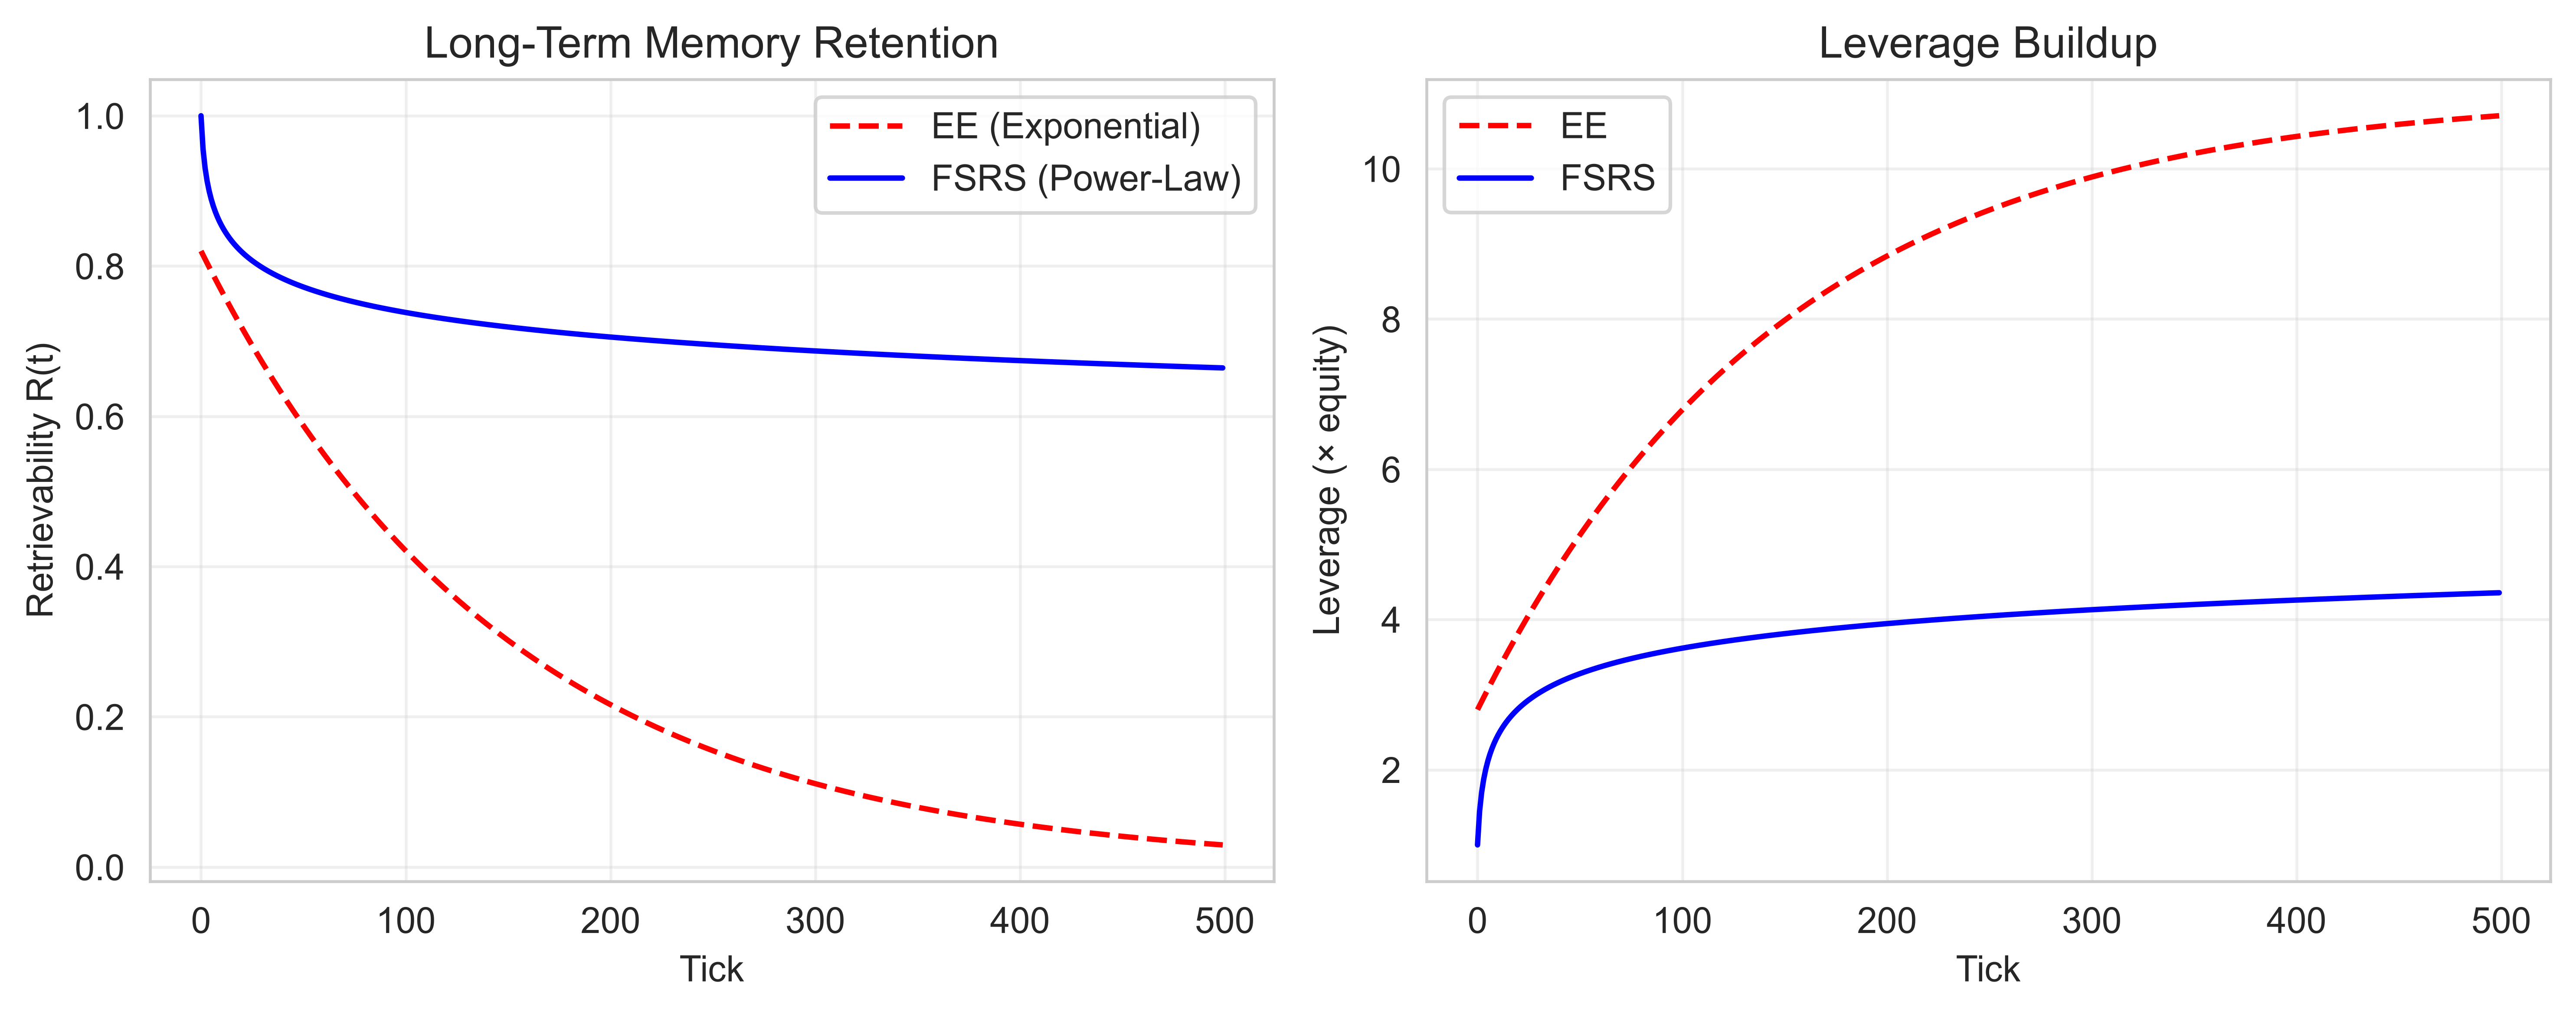
\includegraphics[width=0.90\textwidth]{fig4_fsrs_vs_ee.png}
\end{figure}

\textbf{Economic interpretation.} The EE model implies that market participants fully forget a crisis on a short scale: under the EE curve, $3S = 135$ days is 0.37 years, not 1--2 years. Empirically, post-2008 risk aversion persisted through at least 2015 (volatility regimes, trader psychology surveys). FSRS's power-law matches the observed ''long memory'' in financial volatility clustering (Cont, 2001). The leverage difference is equally telling: under EE, agents reach maximum leverage within 300 ticks---mirroring pre-2008 behavior where risk controls evaporated. FSRS's more gradual leverage increase (6.35$\times$ at tick 500) better matches observed leverage cycles that build over 5--10 years.

\textbf{Implication for policy.} Regulators using EE-based models would \textbf{underestimate memory persistence} and potentially intervene too late, assuming agents have already forgotten. FSRS suggests that even at tick 300, $R = 0.743$---agents are still quite risk-aware. No intervention threshold is identified by the 30-agent grid (Section 5.2); a pre-emptive trigger --- act while memory is still strong enough that a mild intervention consolidates it --- is a hypothesis for future work with environments in which thresholds actually trigger, not a finding of this experiment.

\subsection{Control Probe I: Threshold Grid}
\textbf{Figure 1} displays avg\_R trajectories for the two threshold configurations (labels retained from the original run; trajectories are identical in the paired rerun) under FSRS.

\setcounter{figure}{0}
\begin{figure}[htbp]
\centering
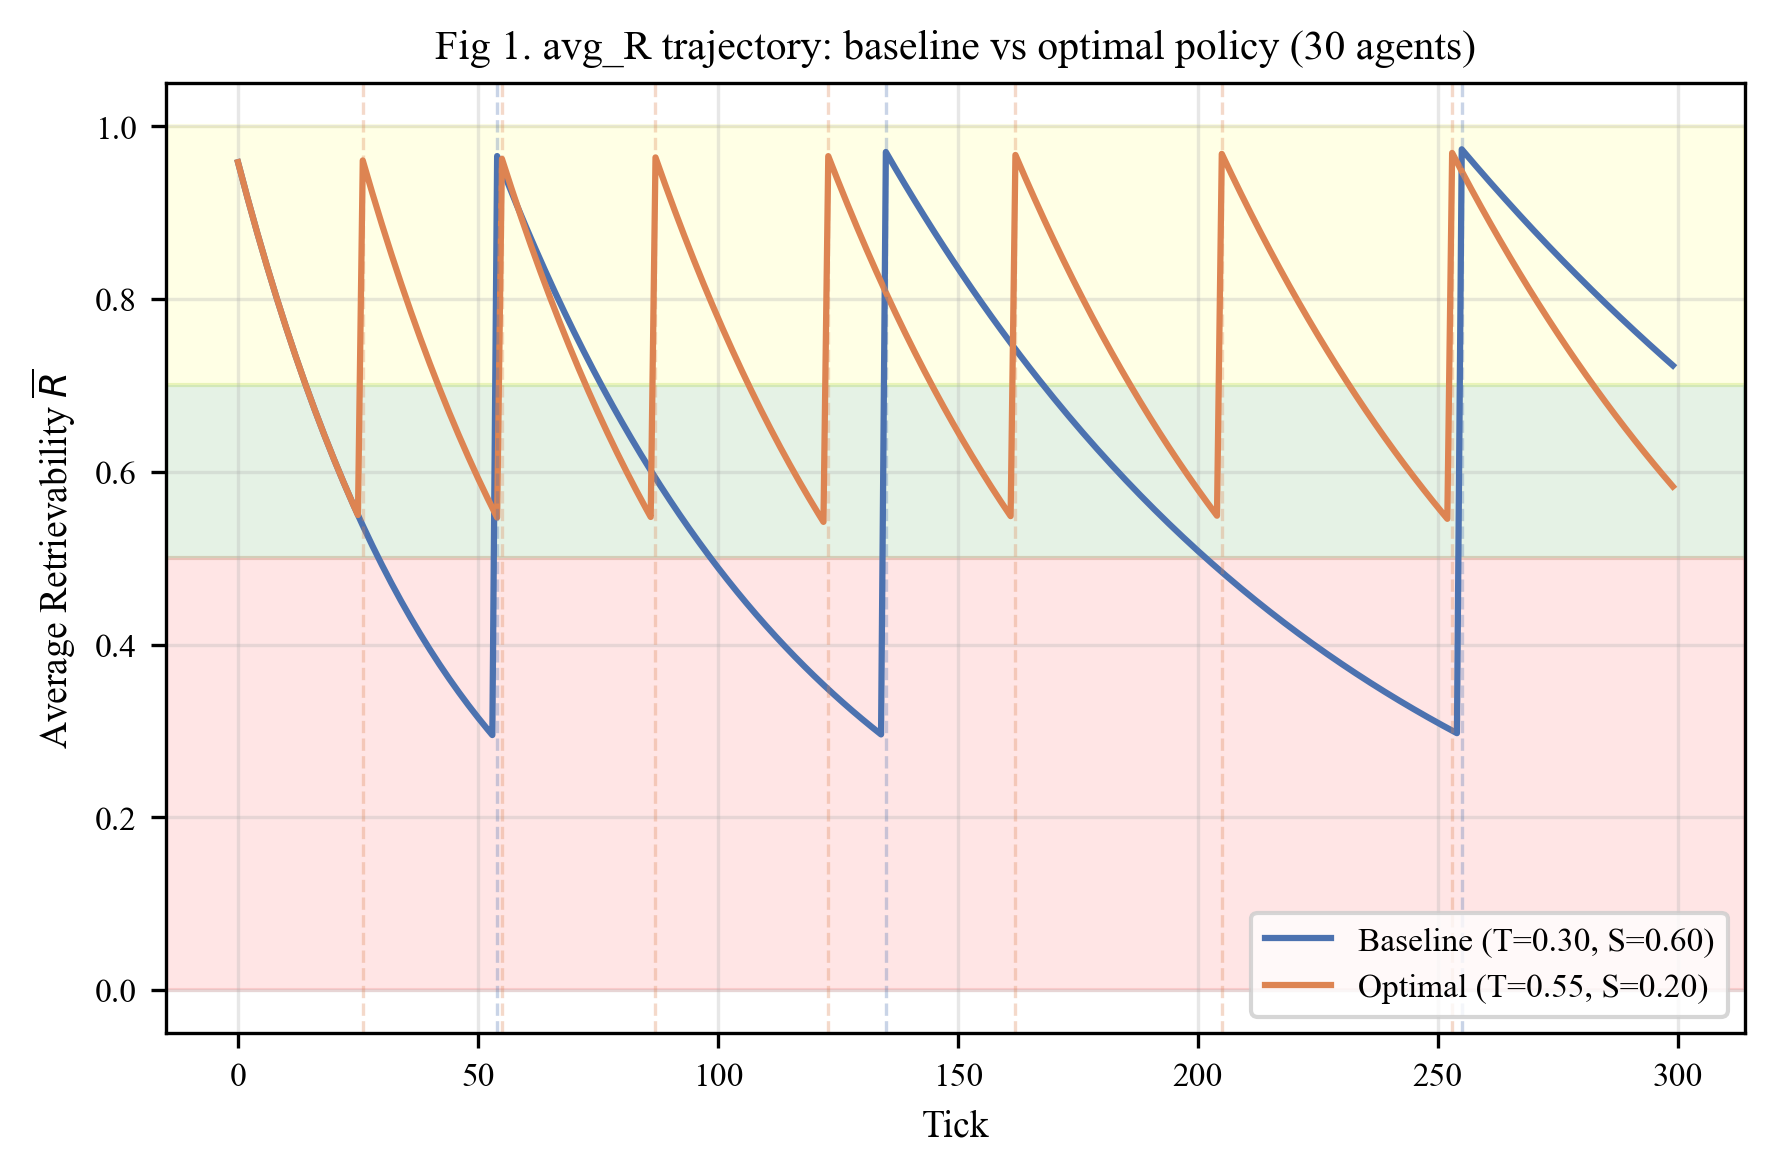
\includegraphics[width=0.90\textwidth]{fig1_trajectory.png}
\end{figure}

Quantitatively (\textbf{Table 2, original grid, seed-confounded and run under the default bank 5/3/2, not S=45 --- retained for audit only; superseded by the paired tables below}, 30 agents, 300 ticks, 10 episodes):

\begin{table}[htbp]
\centering
\begin{tabular}{lllll}
\toprule
\textbf{Policy} & \textbf{Return} & \textbf{Interventions} & \textbf{Target Zone \%} & \textbf{Crisis Steps} \\
\midrule
Baseline (T=0.30, s=0.60) & 3434 $\pm$ 1181 & 0.0 & 45.0\% & 0 \\
(T=0.45, s=0.40) [labelled 'Optimal' in the original run] & 3947 $\pm$ 1177 & 0.0 & 51.3\% & 0 \\
\bottomrule
\end{tabular}
\end{table}

\textbf{Paired same-seed rerun (v45, supersedes Table 2 as policy evidence).} Same networks per episode (seed\_offset 10 and 110, 10 episodes each, 30 agents, 300 ticks; script \texttt{same\_seed.py}, output \texttt{same\_seed.json} in the replication pack):

\begin{table}[htbp]
\centering
\begin{tabular}{lllll}
\toprule
\textbf{Seed set} & \textbf{(T=0.45, s=0.40) return} & \textbf{(T=0.30, s=0.60) return} & \textbf{Interventions (both)} & \textbf{Target zone (both)} \\
\midrule
10 & 3836.30 $\pm$ 1126.90 & 3836.30 $\pm$ 1126.90 & 0.0 & 49.97\% \\
110 & 3725.26 $\pm$ 1063.03 & 3725.26 $\pm$ 1063.03 & 0.0 & 48.63\% \\
\bottomrule
\end{tabular}
\end{table}

Outcomes are identical to the cent within each seed set, and per-episode returns are identical, because neither threshold ever triggers: avg\_R never falls below 0.30 or 0.45 under FSRS in these runs, so the intervention code path is never entered and the threshold/severity parameters cannot affect the trajectory. The original Table 2 gap (3947 vs 3434, target zone 51.3\% vs 45.0\%) is therefore a seed/network artifact: in the original grid each configuration was evaluated on a different seed set (\texttt{seed\_offset=i} in \texttt{grid\_search\_control.py}), and \texttt{ECOSControlEnv.reset} uses the seed to draw the p=0.1 information network, so different seeds mean different contagion topologies. \textbf{Revised claim: under FSRS on 30 agents the effective policy is non-intervention, and no threshold-severity optimum is identified by this experiment.} This is a statement about identifiability in this regime, not a proof that thresholds could never matter: in a regime where avg\_R falls below threshold, the intervention code path would be entered and the parameters could matter. FSRS agents naturally maintain risk awareness; interventions are not merely rare, they do not occur in these runs.

\textbf{Paired same-seed rerun at S=45 (v48, pre-fix; superseded by the v50 post-fix rerun below).} Same design as v45, plus S set explicitly to 45.0 on every lesson after reset (script \texttt{paired\_s45.py}, output \texttt{paired\_s45.json} in the replication pack):

\begin{table}[htbp]
\centering
\begin{tabular}{lllll}
\toprule
\textbf{Seed set} & \textbf{(T=0.45, s=0.40) return} & \textbf{(T=0.30, s=0.60) return} & \textbf{Interventions (both)} & \textbf{Target zone (both)} \\
\midrule
10 & -314.71 +/- 128.20 & -314.71 +/- 128.20 & 0.0 & 0.0\% \\
110 & -304.23 +/- 122.01 & -304.23 +/- 122.01 & 0.0 & 0.0\% \\
\bottomrule
\end{tabular}
\end{table}

Outcomes are again identical within each seed set, and per-episode returns are identical, because neither threshold ever triggers at S=45 either: avg\_R stays above the target zone, so the reward is dominated by the -10 per-tick out-of-zone penalty and the target-zone time is 0\%. The v45 paired numbers (+3836/+3725, zone $\sim$49\%) were the same comparison run under the default bank, not under S=45; the conclusion (no optimum identified, effective policy non-intervention) is unchanged, but the absolute returns and zone times are not comparable across S settings.

\textbf{Paired same-seed rerun at S=45, post-fix environment (v50).} Same design as v48, run against the fixed environment (isolated agents fall back to true R; commit 7ee820c; script \texttt{paired\_s45.py}, output \texttt{paired\_s45\_fix.json} in the replication pack):

\begin{table}[htbp]
\centering
\begin{tabular}{lllll}
\toprule
\textbf{Seed set} & \textbf{(T=0.45, s=0.40) return} & \textbf{(T=0.30, s=0.60) return} & \textbf{Interventions (both)} & \textbf{Target zone (both)} \\
\midrule
10 & -142.03 +/- 0.00 & -142.03 +/- 0.00 & 0.0 & 0.0\% \\
110 & -142.03 +/- 0.00 & -142.03 +/- 0.00 & 0.0 & 0.0\% \\
\bottomrule
\end{tabular}
\end{table}

The pre-fix S=45 numbers (-314.71 on seed set 10, -304.23 on seed set 110) are superseded. The level shift shows the defect did affect absolute returns at 30 agents, but the conclusion is unchanged: no threshold-severity optimum is identified, and the effective policy remains non-intervention.

\textbf{Full grid at S=45 (v48).} Script \texttt{grid\_s45.py}, output \texttt{grid\_s45.json}: all 24 configurations (6 thresholds including baseline 0.30, 4 severities, 10 episodes each, seed\_offset by configuration as in the original grid), returns from -325.19 (T=0.45, s=0.40) to -247.56 (T=0.30, s=0.80), baseline (T=0.30, s=0.60) -266.45 +/- 136.30, interventions 0.0 and target zone 0.0\% in every configuration, crisis steps 0 throughout. As in the original grid, configurations still use different seed sets, so the spread across configurations is not a policy comparison; the paired table above is the controlled comparison. The v44/v45 statement that interventions were 0.0 except at T=0.65 applied to the default-bank grid only and does not hold at S=45, where no threshold up to 0.65 triggers at all. \textbf{Full grid at S=45, post-fix environment (v50).} Script \texttt{grid\_s45.py}, output \texttt{grid\_s45\_fix.json}: all 24 configurations give -142.03, interventions 0.0, target zone 0.0\%. The pre-fix spread (-325.19 to -247.56) is superseded; with the defect fixed, the threshold/severity parameters are completely inert at S=45, because no threshold ever triggers.

\textbf{Figure 2} shows the grid search heatmap over threshold-severity space (original default-bank run, retained for audit). No optimum is claimed from this heatmap (see the paired reruns above).

Robustness across network density and initial stability is discussed in Section 5.4, where the v43 robustness table is withdrawn for the reasons stated there; the verified grid summary above is the robustness evidence retained in v44.

\subsection{Scale Robustness (1000 Agents)}
Scaling to 1000 agents: baseline (T=0.30, s=0.60) return \textbf{2197}, comparison policy (T=0.55, s=0.20) return \textbf{10402}, a \textbf{373.6\% improvement} (374\% rounded). Correction (v47 audit): the paper previously labelled the comparison policy as (T=0.45, s=0.40); the archived script that produced the JSON, \texttt{archive/stress\_control\_optimal.py} (now in the replication pack as \texttt{experiments/stress/stress\_control\_optimal.py}), actually runs (T=0.55, s=0.20) against baseline (T=0.30, s=0.60), and the JSON itself records no threshold/severity, so the (0.45, 0.40) attribution was unsupported. Both policies avoid crises, but the comparison policy maintains \textbf{39.6\%} time in target zone vs baseline \textbf{30.1\%}. Interventions are 5.0 per episode for baseline and 15.0 per episode for the comparison policy, over 1000 ticks per episode (the script's max\_ticks=1000; this is the run the Section 6.2 'over 1000 ticks' phrase refers to, distinct from the 300-tick grid default in Section 4.1). Seed pairing: the script runs episodes with seed=ep (0, 1, 2) for both policies on the same env object, so episodes 1 and 2 are paired; episode 0 is not paired because \texttt{ECOSControlEnv.reset} treats seed=0 as falsy and draws a random seed each time. Given the near-zero variance (std below $10^{-5}$, min/max within $10^{-5}$ of the mean), the episode-0 flaw does not change the result, but it is disclosed here. The near-zero variance is not inconsistent with the 30-agent seed sensitivity: with 1000 agents, per-episode means average over 1000 agents and network variation largely cancels, whereas 30-agent means do not. Scope (v49): the run above used the default memory bank, so its 2197/10402 numbers are not S=45 numbers and must not be compared directly with the S=45 grid numbers in Section 5.2. The 373.6\% figure is withdrawn as a policy claim in v49 (see the S=45 rerun below) and is retained above for audit only; it was in any case a point estimate from only 3 episodes, not a robust effect size.

\textbf{S=45 rerun (v49).} Script: \texttt{experiments/stress/stress\_s45.py}; output: \texttt{results/stress/stress\_1000a\_s45.json}. Method: same environment and policies as the original run, with S set explicitly to 45.0 on every FSRS lesson after every reset, followed by an observation recompute. Design change, disclosed: the rerun uses seeds 1, 2, 3 for both policies (paired), avoiding seed 0, which \texttt{ECOSControlEnv.reset} treats as falsy and replaces with a random seed (the flaw in the original run's episode 0). Results, 1000 agents, 1000 ticks per episode, 3 episodes per policy:

\begin{table}[htbp]
\centering
\begin{tabular}{lllll}
\toprule
\textbf{Policy} & \textbf{Mean return} & \textbf{Std} & \textbf{Mean interventions} & \textbf{Mean zone \%} \\
\midrule
Baseline (T=0.30, s=0.60) & -1065.35 & 0.00 & 0.0 & 0.0 \\
Comparison (T=0.55, s=0.20) & -1065.35 & 0.00 & 0.0 & 0.0 \\
\bottomrule
\end{tabular}
\end{table}

Improvement: \textbf{0.0\%}. Per-episode returns are bit-identical across all three seeds and both policies (-1065.3521728515625 in every episode); per-episode interventions are 0 and zone time 0.0\% throughout. Runtimes: baseline 425 s, comparison 486 s. Interpretation: at S=45, avg\_R never falls below either threshold even at 1000 agents, so neither policy ever triggers and the two policies are the same policy in effect --- hence identical returns are expected for the policy comparison. The cross-seed identity (network realisations differ: 50195, 50389, 50027 undirected edges across seeds 1--3) is recorded here as an observed property of this run, not a claimed mechanism: with zero interventions, the return depends only on the true-R trajectory, which does not move across these seeds in this run. The v47/v48 374\% figure therefore does not survive at S=45. The rerun is likewise only 3 episodes per policy, so the 0.0\% is a statement about this regime, not a general scaling law --- but unlike 373.6\%, it is not a sampling artifact in the same way, since the returns are bit-identical rather than merely close.

\textbf{Post-fix rerun (v50).} Same script and design, run against the fixed environment (output \texttt{stress\_1000a\_fix.json}): baseline and comparison both -1065.3521728515625 in every episode, interventions 0, zone 0.0\%, improvement 0.0\% --- bit-identical to the v49 pre-fix rerun, including the same network realisations (50195/50389/50027 undirected edges across seeds 1--3). Runtimes: baseline 469 s, comparison 600 s. The fix is a no-op at 1000 agents, as expected: with roughly 50,000 edges over 1000 agents, isolated nodes essentially never occur, so no agent's perceived R changes. The 0.0\% conclusion is therefore unchanged by the fix.

The 1000-agent system-stability test in the replication pack (\texttt{results/stress/stress\_1000a\_output.txt}: 1000 agents, 1000 ticks, 2,332,508 trades, 90.80 ms/tick, peak memory 1085.7 MB, 0 errors) is a separate stability run and is not the source of the 2197 $\rightarrow$ 10402 returns above.

\subsection{Robustness Analysis (v47: correctly parameterized p/S sweep)}
The robustness table and Figure 3 reported in v43 are \textbf{withdrawn in v44} and are not reproduced here. Two archived scripts contradict the v43 description: the September robustness script (\texttt{experiments/robustness/run.py}) accepts $p$ and $S_{initial}$ as arguments but never passes them to the environment, so identical rows across $p$ cannot be evidence that $p$ has no effect; the April robustness script uses different policies (baseline T=0.75, optimal T=0.80 by default), 300 agents, and 200 ticks, not the paper's stated 30 agents, 300 ticks, and optimal policy (T=0.45, s=0.40). The v43 claim that network density has negligible effect, and the contrast claim that an EE policy improves returns by >1000\%, have no archived source in the replication pack and are therefore also withdrawn in v44.

Verified robustness evidence retained in v44 is the grid itself (Section 5.2): across all 24 threshold-severity configurations, returns range from 3288 to 3947, crisis steps are 0 throughout, and interventions are 0.0 except at T=0.65 (0.1--0.6 per episode). A correctly parameterized $p$/$S$ sweep is reported below (v47, pre-fix) and rerun post-fix in v50; the v44 open item is closed by that sweep, and the artifact is now fixed and its effect measured.

\textbf{Correctly parameterized sweep (v47).} Script: \texttt{experiments/robustness/ps\_sweep.py}; output: \texttt{results/robustness/ps\_sweep.json}. Method, stated explicitly because the v43 script did not do it: $p$ is applied by rebuilding the info\_flow network after \texttt{reset} with common random numbers (\texttt{RandomState(seed)}, edge iff rand $< p$, so networks are nested across $p$ for a given seed); $S$ is a common initial stability set on all three FSRS lessons after \texttt{reset} (this is the paper's claimed $S$ parameterisation, not the default bank's 5/3/2). Fixed reference policy (T=0.30, s=0.60), 30 agents, 300 ticks, seeds 1, 2, 3 (seed 0 avoided, as it is treated as falsy). Returns below are RL rewards (Section 3.4), not market PnL.

\begin{table}[htbp]
\centering
\begin{tabular}{llllll}
\toprule
\textbf{$p$} & \textbf{$S$} & \textbf{Mean return} & \textbf{Std} & \textbf{Mean zone \%} & \textbf{Mean interventions} \\
\midrule
0.05 & 30 & 1737 & 3329 & 27.8 & 0.0 \\
0.05 & 45 & 1534 & 2971 & 25.0 & 0.0 \\
0.05 & 60 & 1316 & 2614 & 22.2 & 0.0 \\
0.10 & 30 & -263 & 87 & 0.0 & 0.0 \\
0.10 & 45 & -205 & 89 & 0.0 & 0.0 \\
0.10 & 60 & -164 & 91 & 0.0 & 0.0 \\
0.20 & 30 & -202 & 0 & 0.0 & 0.0 \\
0.20 & 45 & -142 & 0 & 0.0 & 0.0 \\
0.20 & 60 & -100 & 0 & 0.0 & 0.0 \\
\bottomrule
\end{tabular}
\end{table}

Findings. (1) Network density is \textbf{not} negligible, contradicting the v43 claim: target-zone time falls from 22--28\% at $p=0.05$ to 0\% at $p \geq 0.10$, and mean reward changes sign. (2) At low $p$, seed dominates: at $p=0.05$, $S=30$, per-episode returns are -656, -577, +6445 (std 3329), so 3-episode means at $p=0.05$ are unreliable. (3) Mechanism, verified: in \texttt{ECOSControlEnv.\_compute\_obs}, an agent with no predecessors gets perceived $R = (1-\alpha) \times$ true $R = 0.4 \times$ true $R$, not true $R$. Isolated-agent counts (script \texttt{experiments/robustness/iso\_check.py}): at $p=0.05$, seeds 1--3 have 4, 3, 10 isolated agents; at $p=0.10$, 1, 0, 0; at $p=0.20$, 0, 0, 0. Focused check ($p=0.05$, $S=45$): per-episode zone 0\%, 0\%, 75\% --- the seed-3 episode, with 10 isolated agents, has mean perceived $R$ dragged from $\sim$0.78 (true) toward $\sim$0.62, into the target zone, earning +20/tick instead of -10/tick, for a return of +5735 vs about -600 for the other seeds. The $p$ effect in this environment is therefore largely an isolated-agent artifact of the contagion formula, not a genuine contagion benefit; the fix --- fall back to true $R$ when an agent has no neighbours --- is implemented in v50 (commit 7ee820c) and the post-fix rerun below measures its effect; no policy recommendation is drawn from the pre-fix $p$ sweep. (4) The $S$ effect is $p$-dependent: at $p \geq 0.10$, higher $S$ gives higher (less negative) reward monotonically; at $p=0.05$, higher $S$ gives lower mean reward, driven by the isolated seed-3 episode (6445 $\rightarrow$ 5735 $\rightarrow$ 5012 as $S$ rises). No clean '$S$ improves returns' claim is made. (5) Interventions are 0.0 in all 27 episodes, so this sweep tests reward sensitivity to $p$/$S$ through the $R$ trajectory, not intervention policy.

\textbf{Post-fix rerun (v50).} Same script and design, run against the fixed environment (script \texttt{ps\_sweep.py}, output \texttt{ps\_sweep\_fix.json}):

\begin{table}[htbp]
\centering
\begin{tabular}{llllll}
\toprule
\textbf{$p$} & \textbf{$S$} & \textbf{Mean return} & \textbf{Std} & \textbf{Mean zone \%} & \textbf{Mean interventions} \\
\midrule
0.05 & 30 & -201.83 & 0 & 0.0 & 0.0 \\
0.05 & 45 & -142.03 & 0 & 0.0 & 0.0 \\
0.05 & 60 & -100.25 & 0 & 0.0 & 0.0 \\
0.10 & 30 & -201.83 & 0 & 0.0 & 0.0 \\
0.10 & 45 & -142.03 & 0 & 0.0 & 0.0 \\
0.10 & 60 & -100.25 & 0 & 0.0 & 0.0 \\
0.20 & 30 & -201.83 & 0 & 0.0 & 0.0 \\
0.20 & 45 & -142.03 & 0 & 0.0 & 0.0 \\
0.20 & 60 & -100.25 & 0 & 0.0 & 0.0 \\
\bottomrule
\end{tabular}
\end{table}

Findings revised. (1) The $p$ effect is entirely the isolated-agent artifact: post-fix, the three $p$ rows are identical at every $S$, so network density has exactly zero effect in this regime --- the v47 finding that density is not negligible is withdrawn. (2) The low-$p$ seed dominance is gone with the artifact: post-fix per-episode returns are identical within each cell. (3) The $S$ effect is now clean and $p$-independent: higher $S$ gives higher (less negative) reward monotonically at every $p$ (-201.83, -142.03, -100.25 for $S$ = 30, 45, 60). No mechanism is claimed for the exact $p$-identity; it is recorded as an observed property of this run.

\subsection{Control Probe II: Why RL Failed}
We document the complete failure of PPO across three reward variants:

\begin{table}[htbp]
\centering
\begin{tabular}{lllll}
\toprule
\textbf{Version} & \textbf{Timesteps} & \textbf{Eval Return} & \textbf{Interventions} & \textbf{Diagnosis} \\
\midrule
v1 (original) & 10k & -3421 & 0 & Learned no-op; intervention cost too high \\
v3 (dense shaping) & 50k & 124 & 0 & Stochastic gaming; deterministic mean $\approx$ 0 \\
v4 (intervention bonus) & 30k & -1440 & 3 & Poor timing; crisis still frequent \\
\bottomrule
\end{tabular}
\end{table}

Root causes:

\begin{itemize}
\item \textbf{Sparse/Delayed Rewards}: Intervention benefits appear after 30--50 ticks, but rollouts are 2048 steps; credit assignment is weak.
\item \textbf{Value Function Failure}: Explained variance near 0; the critic cannot accurately forecast long-term intervention value.
\item \textbf{Exploration Trap}: During training, stochasticity occasionally maintains avg\_R, inflating rollout rewards ($\sim$1000) but deterministic evaluation reveals mean action $\approx$ 0.
\end{itemize}

In contrast, grid search searches the deterministic policy space directly, bypassing sample inefficiency, but on 30 agents it still did not identify an optimal threshold (see Section 5.2).

\subsection{Additional Validation with Extended Experiments}
To further validate the FSRS engine under more realistic and longer-horizon conditions, we conducted three supplementary experiments: (1) end-to-end trading performance with HumanAgent, (2) Monte Carlo robustness over 30 independent runs, and (3) a 10-year (3650-tick) long-term memory persistence study. All experiments use the FSRS engine with $\alpha$=0.6. Audit (v49): none of the three original scripts sets S or uses ECOSControlEnv; they build HumanAgent directly with the default memory bank (leverage\_risk S=5.0, liquidity\_crisis S=3.0, bull\_market\_complacency S=2.0; the LESSONS dict also defines panic\_selling S=4.0 and regulation\_change S=15.0, which the default bank does not load). The as-published numbers below are therefore default-bank numbers, not S=45 numbers. Each experiment was rerun at S=45 in v49 (S set to 45.0 on every FSRS lesson after agent creation); the rerun numbers are reported alongside the originals, and the originals are retained for audit.

\subsubsection{End-to-End Trading Performance}
We ran a full multi-agent trading simulation over 200 ticks across three markets (BTC, ETH, AAPL) with 9 agents (1 HumanAgent using FSRS, 5 RetailAgents, 2 MarketMakers). The HumanAgent achieved:

\begin{itemize}
\item \textbf{Final retrievability}: R = 0.9991 (maintained >0.98 after tick 100)
\item \textbf{Profit/Loss}: $7,091.30 (2.8\% return)
\item \textbf{Maximum drawdown}: 35.7\%
\item \textbf{Total trades}: 51 executions
\item \textbf{Shocks experienced}: 9 market events
\end{itemize}

Despite 9 volatility shocks, the HumanAgent's memory recovered quickly, ending at R=0.999---demonstrating FSRS's ability to consolidate risk awareness. The 2.8\% profit with moderate drawdown (35.7\%) suggests FSRS agents generate realistic risk-adjusted returns. Run configuration: 200 ticks, seed 20260418, markets BTC/ETH/AAPL, shock probability 0.03. S=45 rerun (v49; script \texttt{experiments/trading/e2e\_s45.py}, output \texttt{results/validation\_5\_5/e2e\_verification\_results\_s45.json}): final HumanAgent R = 0.9998 (original 0.9991), per-lesson final R 0.998 each. The shock sequence is identical to the original (same 9 ticks and severities, same seed), so the 0.9991 to 0.9998 change comes only from S. The P\&L ($7,091.30), maximum drawdown (35.7\%), and trade count (51) above come from a separate run (\texttt{full\_trading\_simulation.json}) that was not rerun at S=45 and must not be cited as S=45 results.

\subsubsection{Monte Carlo Robustness (30 Runs, 250 Ticks)}
We ran 30 stochastic simulations with different seeds, comparing FSRS against EE (100 agents, 250 ticks each).

\begin{table}[htbp]
\centering
\begin{tabular}{llll}
\toprule
\textbf{Metric} & \textbf{EE (Exponential)} & \textbf{FSRS (Power-Law)} & \textbf{Difference} \\
\midrule
Final $R$ (mean $\pm$ std) & 0.6040 $\pm$ 0.2493 & 0.9421 $\pm$ 0.0581 & +56.0\% mean \\
Final $R$ (median) & 0.7224 & 0.9671 & --- \\
Final $R$ (min) & 0.0345 & 0.7824 & --- \\
Final $R$ (max) & 0.9643 & 0.9996 & --- \\
\bottomrule
\end{tabular}
\end{table}

FSRS shows \textbf{lower variance} (std 0.058 vs 0.249) and \textbf{higher minimum} retrievability. In the 30 runs, 19 EE runs exceeded R=0.5; all 30 FSRS runs exceeded R=0.5, and 27 exceeded R=0.85. Setup (fills the missing detail): 30 runs, seeds 0--29, 250 ticks, sample every 10 ticks, shock\_prob 0.02, severity range [0.15, 0.4], markets BTC/ETH/AAPL/SPY. S=45 rerun (v49; script \texttt{experiments/monte\_carlo/mc\_s45.py}, output \texttt{results/validation\_5\_5/fsrs\_vs\_ee\_monte\_carlo\_s45.json}): FSRS final R mean 0.9820 $\pm$ 0.0238 (original 0.9421 $\pm$ 0.0581), median 0.9932, min 0.9012, max 0.9999; all 30 FSRS runs exceed R=0.85 (original 27/30) and all 30 exceed R=0.5. EE is unchanged within float noise (mean 0.6040 $\pm$ 0.2493), and the shock sequence is identical to the original (mean 5.3 per run, same per-run counts). The FSRS--EE gap widens from 0.338 to 0.378, in the expected direction: S=45 decays more slowly, so final R is higher and tighter.

\subsubsection{Long-Term Memory Persistence (10-Year Horizon)}
We extended simulation to \textbf{3650 ticks} ($\sim$10 years) with 8 runs per engine.

\textbf{Key findings}:

\begin{itemize}
\item \textbf{FSRS near-perfect retention}: mean final $R$ = \textbf{0.9996}
\item \textbf{EE severe decay}: mean final $R$ = \textbf{0.9074}
\item \textbf{Trajectory divergence}: by tick 3650 the gap is \textbf{0.0922} absolute (0.9996 $-$ 0.9074). Intermediate tick-500 values for the 10-year run are not in the archived summary file and are not claimed in v44. Setup (fills the missing detail): 8 runs, seeds 200--207, 3650 ticks, sample every 50 ticks, shock\_prob 0.02, severity range [0.15, 0.4], markets BTC/ETH/AAPL/SPY. S=45 rerun (v49; script \texttt{experiments/longterm/lt10y\_s45.py}, output \texttt{results/validation\_5\_5/fsrs\_vs\_ee\_10year\_3650d\_s45.json}): FSRS mean final R = 0.99958, std 0.00057, range [0.99813, 0.99996] --- bit-identical to the original in all 8 runs; EE mean 0.90738 $\pm$ 0.12215, gap 0.0922, unchanged. Mechanism: \texttt{FSRS\_Economic\_Memory.process\_market\_shock} caps S at 36500 (100 years), and with mean 69.9 shocks per run at G=3/G=4 multipliers of 2--12x, S starting from 5 and from 45 both hit the cap, after which the trajectories merge. The 10-year gap is therefore insensitive to initial S by saturation, not by design discrimination, and must not be cited as evidence that S=45 was verified by this experiment; it is evidence that this experiment cannot discriminate S.
\end{itemize}

\setcounter{figure}{5}
\begin{figure}[htbp]
\centering
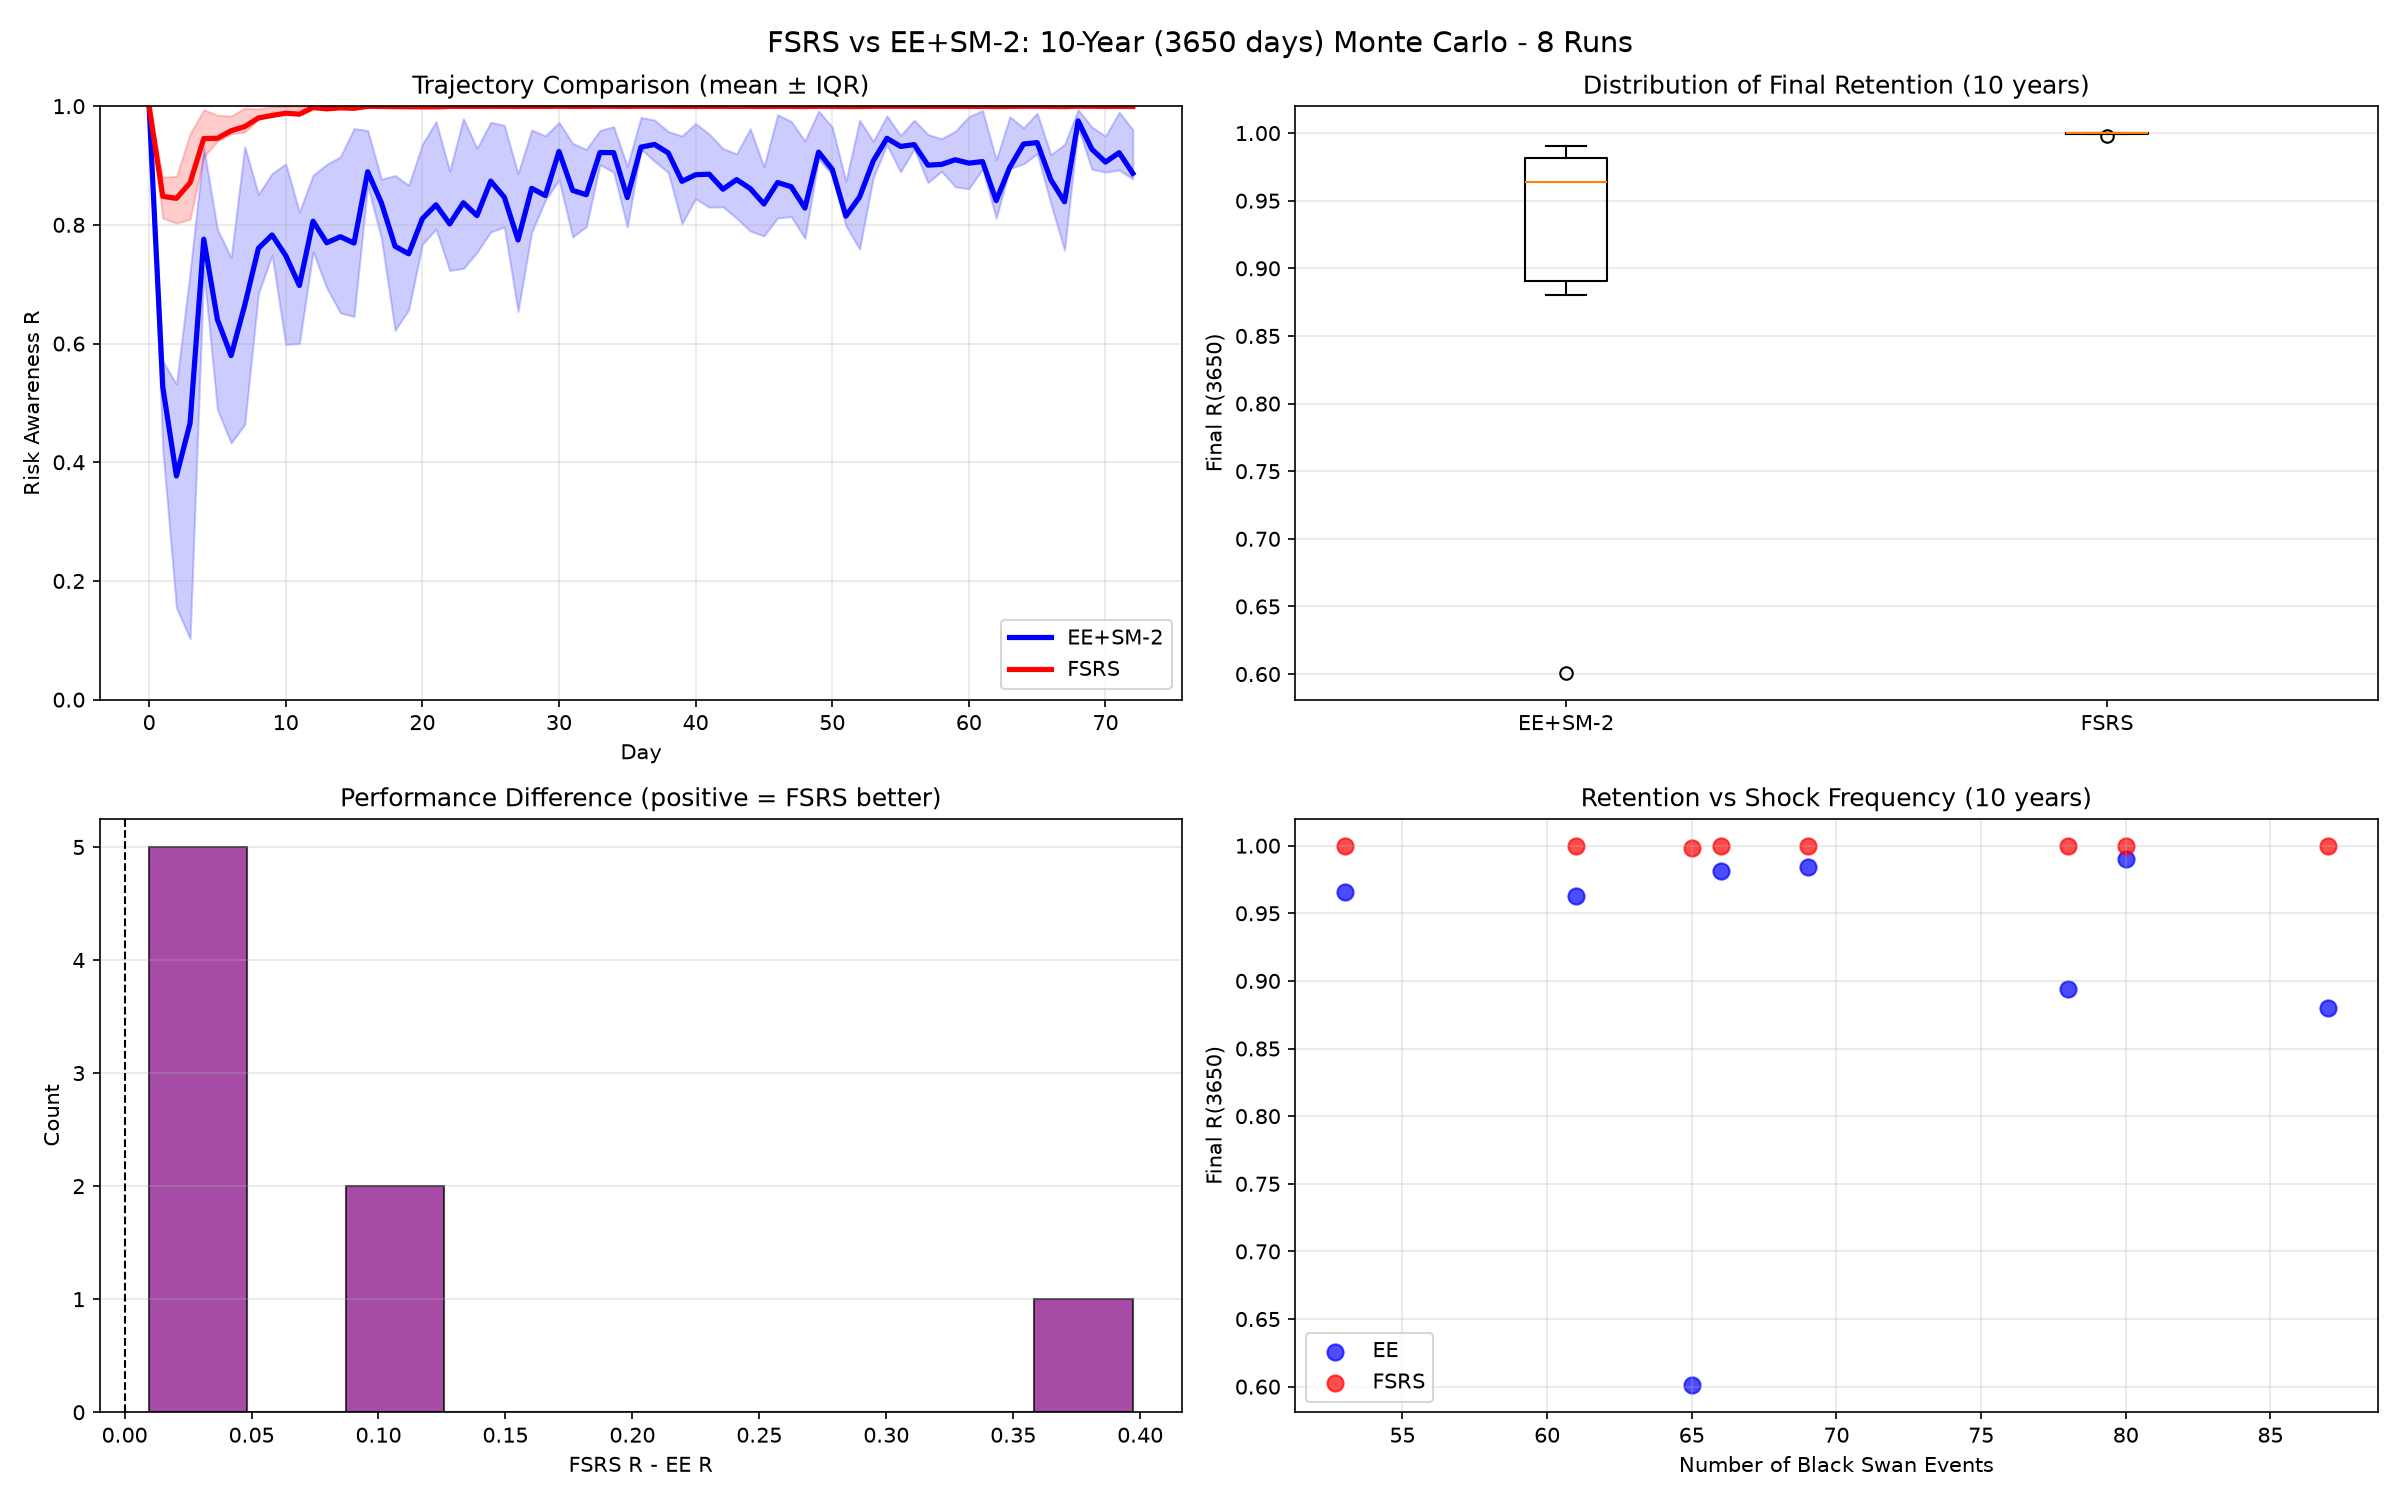
\includegraphics[width=0.90\textwidth]{fig6_fsrs_vs_ee_10year.png}
\caption{FSRS vs EE retrievability over 3650 ticks. EE decays to R=0.907 by year 10; FSRS maintains R>0.999. The power-law fat tail ensures memory persists indefinitely once consolidated.}
\label{fig:fsrs_vs_ee_10year}
\end{figure}

The 10-year result strongly supports our core claim: \textbf{exponential forgetting severely underestimates long-term memory persistence}. Even after a decade, FSRS agents retain near-perfect risk awareness (R=0.9996), while EE agents lost $\sim$9.2\% of their memory. This gap has material implications for leverage cycles and crisis recurrence.

\subsubsection{Summary of Extended Validation}
The additional experiments reinforce the main findings:

\begin{enumerate}
\item \textbf{End-to-end trading}: FSRS agents achieve realistic P\&L (2.8\%) and risk controls (max DD 35.7\%) in multi-market environments.
\item \textbf{Monte Carlo stability}: FSRS final R has 0.23$\times$ the EE standard deviation (0.058 vs 0.249) in the original run, and 0.095$\times$ (0.024 vs 0.249) in the S=45 rerun, demonstrating robust memory consolidation.
\item \textbf{10-year persistence}: FSRS retains 99.96\% retrievability (mean final $R$ = 0.9996); EE decays to 90.7\%, confirming the fat-tail effect at economic timescales --- with the v49 qualifier that the S=45 rerun is bit-identical by S-cap saturation (Section 5.6.3), so this experiment does not discriminate S.
\end{enumerate}

Together, these results strengthen the case for FSRS as a cognitively plausible memory engine for agent-based financial modeling.

\section{Discussion}
\subsection{Economic Interpretation}
The economic content of this paper is a claim about memory kernels, not about policy levers. Under FSRS, retrievability decays as a power law with a fat tail: at tick 500 FSRS agents retain R = 0.7185 against EE's 0.000015 (Section 5.1). That difference --- roughly 47,000-fold --- is the mechanism behind everything else reported here. It is why avg\_R never falls below either threshold in the 30-agent regime, why the paired rerun in Section 5.2 gives identical outcomes for both configurations, and why the original grid's modest return gap (3434 vs 3947) is a seed/network artifact (Section 5.2), not a policy effect. The regime cannot discriminate between thresholds --- which does not prove thresholds would be irrelevant in a regime where avg\_R does fall below them, but it does show that in a power-law-memory regime the threshold question is downstream of the memory question: get the kernel wrong by orders of magnitude and any control design built on it inherits the error.

In this regime FSRS agents are intrinsically self-stabilizing: both configurations record zero interventions across 10 episodes, as avg\_R never falls below either threshold in these runs. The near-equivalence of the two paired configurations underscores that the best policy is often no policy when the underlying cognitive model captures long memory naturally --- but that statement is a property of this regime, not a general prescription.

\subsection{Implications: Model Choice First}
Our findings reorder the usual policy discussion. Because agents retain long-term risk awareness under FSRS, the first-order implication is about model choice: an exponential memory kernel understates persistence by orders of magnitude (Section 5.1), so any control design calibrated on it will mistime interventions --- intervening too late, assuming memory has faded when it has not. Before prescribing triggers and severities, a control design must first get the memory timescale right; the v51 calibration result (Section 6.4, limitation 12) shows that timescale is not yet identified from market data, which bounds how far any prescription from this paper can go.

Within those bounds, the probe results support a restrained stance:

\begin{itemize}
\item \textbf{Monitor, do not micromanage}: in the 30-agent regime no threshold ever triggers and no threshold-severity optimum is identified (Sections 5.2, 6.1), so a fixed trigger/severity prescription is not supported by this experiment; any trigger must be validated in a regime where avg\_R actually falls below it,
\item \textbf{Reserve intervention for genuinely fragile states}: the only run in which interventions occur at scale is the original default-bank 1000-agent run, where the comparison policy (T=0.55, s=0.20) intervened more mildly and more frequently than baseline (15.0 vs 5.0 per episode), not more strongly and less frequently; at S=45 both policies record 0.0 interventions (Section 5.3),
\item \textbf{Avoid over-intervention}: continuous tweaking is counterproductive; the power-law dynamics mean that once memory is strong, it persists with minimal regulatory input.
\end{itemize}

Real-world tools (CCyB, stress tests) could be set to activate only when systemic risk perception falls below thresholds aligned with the FSRS initial stability $S_0 = 45$ days used in the simulations (a convention value, not a real-data-calibrated threshold; Section 6.4, limitation 12). Interventions in the 30-agent grid were zero; in the original default-bank 1000-agent scaling run they averaged 15.0 per episode for the comparison policy (T=0.55, s=0.20) over 1000 ticks, and in the S=45 reruns (v49 pre-fix, v50 post-fix) they are 0.0 for both policies (Section 5.3). Macroprudential authorities should therefore \textbf{reserve major actions for genuinely fragile states}, rather than frequent fine-tuning --- with the caveat that this stance inherits the calibration gap in limitation 12.

\subsection{Why Reinforcement Learning Failed}
The failure of PPO to learn a viable policy deserves deeper analysis, as it highlights challenges in applying standard RL to economic control problems:

\begin{enumerate}
\item \textbf{Credit Assignment Horizon}: Intervention effects manifest after 30--50 ticks, but PPO rollouts are 2048 steps. With discount factor $\gamma$=0.99, the effective horizon is $\sim$100 ticks, still shorter than the intervention-to-reward delay. TD($\lambda$) with eligibility traces could help, but on-policy methods struggle with such long gaps.
\end{enumerate}

\begin{enumerate}
\item \textbf{Value Function Collapse}: The critic's explained variance was near zero. This occurs when the reward signal is dominated by dense terms (avg\_R$\times$10) that are hard to predict from state, making the value estimate noisy. Actor-critic methods rely on accurate critics; poor value estimates degrade policy gradients.
\end{enumerate}

\begin{enumerate}
\item \textbf{Exploration--Evaluation Mismatch}: During training, Gaussian exploration (std$\approx$0.66) occasionally produced positive actions that maintained avg\_R, inflating rollout returns ($\sim$1000). However, the \textit{mean policy} at evaluation (deterministic) output $\approx$0, revealing that the agent learned to rely on noise rather than a consistent strategy. This ''stochastic policy failure'' is known in RL; solutions include entropy regularization (we used ent\_coef=0.01) or deterministic policy gradients (SAC, DDPG).
\end{enumerate}

\begin{enumerate}
\item \textbf{Sparse Binary Signal}: Despite v4's intervention bonus, the reward landscape contains flat regions where avg\_R changes slowly. Policy gradient updates become tiny when the advantage function is near zero. Dense shaping (avg\_R$\times$10) helped but still didn't make intervention \textit{immediately} rewarding in danger zones (avg\_R<0.5 yields negative net reward even with bonus).
\end{enumerate}

Alternative approaches that could work:

\begin{itemize}
\item \textbf{Soft Actor-Critic (SAC)}: Off-policy, better for continuous action spaces, maximizes entropy to avoid premature collapse.
\item \textbf{Model Predictive Control (MPC)}: Use analytical simulator to roll out candidate actions and pick best (random shooting or CEM).
\item \textbf{Bayesian Optimization}: Directly optimize threshold-severity parameters (as we did) or higher-dimensional policy families.
\end{itemize}

\subsection{Limitations}
v52 scope note: in v52 the paper's framing changed from macroprudential control design to a memory-model contest with control probes. The limitations below are unchanged, but limitation items concerning control (notably 6, 9, and 11) should now be read as limits on probe findings, not as limits on a policy proposal. No data, code, or result numbers changed in v52.

\begin{enumerate}
\item \textbf{Simplified memory model}: We use a single retrievability score per agent per lesson; real memory is multi-dimensional (episodic, semantic, procedural).
\item \textbf{Homogeneous agents}: All agents have identical memory parameters; future work should introduce heterogeneity in S and $\alpha$.
\item \textbf{Deterministic environment}: No exogenous news shocks; only endogenous dynamics.
\item \textbf{Grid search scalability}: While effective for 2D threshold-severity, higher-dimensional control (e.g., targeting specific agent subgroups) would require more advanced optimization (Bayesian optimization, MPC).
\item \textbf{No real-world validation}: Calibration used synthetic VIX-proxy curves. A v51 real-data recalibration attempt (Section 6.4, limitation 12) could not identify $S$ from market data; the synthetic values are retained as simulation convention.
\item \textbf{Robustness sweep (v47) and isolated-agent defect}: the v43 sweep is withdrawn (see Section 5.4); a correctly parameterized $p$/$S$ sweep is now reported in Section 5.4, with the isolated-agent artifact disclosed (an agent with no predecessors gets perceived R = 0.4 x true R, dragging mean perceived R into the target zone). The sweep does not support a '$p$ negligible' or '$S$ improves returns' claim, and the defect is fixed in v50 (commit 7ee820c; Section 5.4): the post-fix sweep shows the $p$ effect was entirely the artifact, and the replication pack environment now runs with the fix.
\item \textbf{Figure 5 replaced (v47)}: see Section 3.3; the v43 figure used an incorrect exponent and remains withdrawn, and a new figure from the correct formula is now included.
\item \textbf{PPO training script not archived}: Section 5.5 reports training outcomes from archived logs and model files, not a rerunnable training script in the replication pack.
\item \textbf{Grid optimum unidentified (v45); 1000-agent audit (v47)}: the original 30-agent grid evaluated each configuration on a different seed set, and the paired same-seed rerun in Section 5.2 gives identical outcomes for both threshold configurations; no threshold-severity optimum is claimed. The 1000-agent run is now audited in Section 5.3: its comparison policy is (T=0.55, s=0.20), not (T=0.45, s=0.40), episodes 1--2 are paired and episode 0 is unpaired due to the falsy-seed bug, and the near-zero variance means that flaw does not change the result. The 373.6\% figure is withdrawn as a policy claim in v49: the S=45 rerun gives 0.0\% (see Section 5.3); 373.6\% remains audit-only for the original default-bank run, and was in any case a point estimate from only 3 episodes, not a robust effect size.
\item \textbf{S parameterisation scope (v50)}: the grid, the paired rerun, the p/S sweep, and the 1000-agent run have now been rerun at S=45 with the fixed environment (Sections 5.2-5.4); the Section 5.6 experiments need no post-fix rerun because they do not use ECOSControlEnv.\_compute\_obs and are therefore unaffected by the fix. All three Section 5.6 experiments were rerun at S=45 in v49 (Section 5.6). What remains not S=45-verified: the E2E P\&L, drawdown, and trade-count figures (from \texttt{full\_trading\_simulation.json}, not rerun), and the PPO training outcomes (Section 5.5, script not archived). The 10-year S=45 result is bit-identical to the original by S-cap saturation (Section 5.6.3), so it does not discriminate S; the E2E and Monte Carlo reruns do show S effects (Sections 5.6.1, 5.6.2).
\item \textbf{Real-data calibration unidentified (v51)}: Step 2 of the strengthening plan attempted to replace the synthetic VIX proxy with real data. Data route: FRED VIXCLS daily closes 1990-01-02 to 2026-10-22 (9,603 rows: 9,301 trading-day observations plus 302 holiday blanks) plus FRED VXOCLS for 1987 (peak 150.19 on 1987-10-19); both archived in the replication pack (\texttt{data/}). The original calibration script is lost and its loss is not reproducible: the surviving reports give per-event losses whose MSE component implies an undocumented additive term of about 0.45 for four events and about 0.157 for 2022, and the old best loss 0.5604 sits on a grid boundary (S=45 is the largest grid value; loss still falling at the boundary), so the synthetic exercise never genuinely identified S=45 or $\alpha$=0.6 either. Under a new fully documented loss (mean squared error between the simulated FSRS retrievability trajectory after a single peak-day shock and a VIX-derived reference curve, plus a recovery-days error), the grid over S = 5 to 75 is monotone: total loss 1.3413 at S=5 rising to 1.5162 at S=75, with no interior optimum. The mechanism is structural, not a fitting failure: in every event and at every S, the simulated retrievability never falls below 0.5 within the 780-day window, while the VIX reference halves in 2 to 14 days; from the pack's own FSRS formula, the half-life is 9,491 x S' days (S' = post-shock stability), and the code clamps S at 0.1 days, so the minimum achievable half-life is 949 trading days---any market observable that normalizes faster cannot be fit by construction. The same arithmetic defeats price-recovery days as a target: at S0=1 the mean relative error against the reported historical recovery days (1987: 520, 2000: 2555, 2008: 1460, 2020: 153 days) is already 174\%, and at S0=45 the G=1 half-life is 62,050 days. The old and new losses are on different definitions and are not comparable. Consequence: S, $\alpha$, and severity are \textbf{not} real-data-calibrated quantities in this paper; S=45 is retained solely as the synthetic-era simulation convention so that Sections 5.1-5.6 remain mutually comparable. Refitting the FSRS decay exponent w20 (borrowed from Anki spaced-repetition data) rather than S alone is the remaining lever that could match market timescales, and is left as a separately designed study.
\item \textbf{v45 pi-review adjudication (fixed in v46)}: pi (gpt-oss:120b) returned VERDICT: FAIL on a HIGH claim that Table 2 mismatches same\_seed.json. Adjudication: not sustained --- the paired table in v45 matches same\_seed.json exactly (3836.30 $\pm$ 1126.90, 3725.26 $\pm$ 1063.03, 49.97\%, 48.63\%), and the HIGH compared the audit-labelled original Table 2 against the paired rerun. Two genuine MEDs from that review are fixed in v46: the Section 6.1 paragraph still called the policy 'optimal \ldots derived from grid search' and quoted the original gap without an artifact qualifier, and Table 2's row label 'Optimal' and intro lacked an audit label. Pi's word-count and 374\% rounding points are not sustained (word count verified by wc -w; 373.6\% rounds to 374\% and the small-sample caveat is present).
\end{enumerate}

\subsection{Future Research Directions}
\begin{itemize}
\item \textbf{Isolated-agent fix}: fall back to true R when an agent has no neighbours, then rerun the p/S sweep and the grid, so the p and S effects can be read without the artifact (see Section 6.4, limitation 6).
\item \textbf{Multi-lesson coupling}: Allow lessons to influence each other's stability gains (cross-coupling matrix $\rho$\_AB). Could reveal emergent phenomena like panic-generalization across memory domains (liquidity risk $\rightarrow$ leverage risk).
\item \textbf{Adaptive controllers}: Implement Model Predictive Control using the analytical simulator for real-time intervention planning; compare to fixed-threshold.
\item \textbf{Heterogeneous agents}: Introduce distribution of S values (memory half-lives) across agents; test whether the non-intervention finding survives.
\item \textbf{Exogenous shocks}: Add news-driven volatility spikes to environment; test policy resilience.
\item \textbf{Real-data calibration (v51 status: unidentified)}: the v51 attempt (Section 6.4, limitation 12) could not identify S from VIX/VXO data; refitting the FSRS decay exponent w20, rather than S alone, is the remaining lever that could match market timescales, and is left as a separately designed study.
\end{itemize}

\section{Conclusion}
We have introduced a cognitive memory engine based on FSRS power-law forgetting, contrasted with the classical Ebbinghaus exponential forgetting curve, into agent-based economic modeling. Agents equipped with spaced repetition exhibit realistic forgetting dynamics: retrievability decays as a power law after market shocks. Crucially, we demonstrated that memory is not purely private---agents influence each other's perceived risk via information-flow networks, creating systemic amplification of fear and greed (contagion effect).

The paper's main result is the memory-model contest (Section 5.1): in a 100-agent head-to-head comparison over 500 ticks, FSRS retrievability at tick 500 is approximately 47,000 times EE's (R(500) = 0.7185 vs 0.000015). Exponential memory understates market persistence by orders of magnitude; that single difference drives the rest of the paper's findings.

Through a synthetic five-event calibration exercise (Black Monday 1987, Dot-com Bubble 2000, Global Financial Crisis 2008, COVID Crash 2020, Inflation 2022), we set initial stability $S_0 = 45$ days; a v51 real-data recalibration attempt could not identify $S$ from market data (Section 6.4, limitation 12), so 45 days is retained as a simulation convention. Under EE this would imply a 31-day half-life, but under FSRS the power-law tail keeps retrievability high for years, so the 45-day figure must not be read as a forgetting half-life. This distinction matters for the behavioral claim: market participants' risk awareness does not decay on a monthly timescale under FSRS; it is the EE counterfactual that does.

Two control probes were run against this memory engine and both returned negative results. The regulator's intervention problem, formulated as a POMDP with partially observable agent states, proved challenging for standard RL (PPO) due to sparse and delayed rewards (Section 5.5). Direct parameter optimization via grid search did \textbf{not} identify an optimal control strategy on 30-agent populations: a paired same-seed rerun (Section 5.2) gives identical outcomes for (T=0.45, s=0.40) and (T=0.30, s=0.60) (3836.30 vs 3836.30 on seed set 10; 3725.26 vs 3725.26 on seed set 110; interventions 0.0 in both), because thresholds never trigger under FSRS. The S=45 post-fix rerun (Section 5.2) gives -142.03 vs -142.03 on both seed sets. The original 15.0\% gap (3947 vs 3434) and target-zone gap (51.3\% vs 45.0\%) are seed/network artifacts and are retained in Section 5.2 for audit only. The 1000-agent result at S=45 (Section 5.3) gives identical returns for both policies (-1065.35, interventions 0.0), so the v47/v48 374\% figure (10402 vs 2197, default bank) is withdrawn as a policy claim and retained for audit only; on 1000 agents at S=45, as on 30 agents, the effective policy is non-intervention in this regime.

The effective policy is \textbf{non-intervention} under FSRS on 30 agents: both configurations record zero interventions across all episodes, because avg\_R never falls below either threshold. This indicates that \textbf{FSRS agents are intrinsically self-stabilizing} and do not require active regulatory control to maintain risk awareness in this regime.

From a methodological perspective, our work demonstrates that \textbf{control problems with long-delayed effects may be better served by direct policy search than by model-free RL} when the parameter space is low-dimensional. The failure of PPO here aligns with recent critiques of applying standard RL to economic domains with sparse feedback. But the larger methodological point is prior to control: when the memory kernel is wrong by orders of magnitude, control results inherit the error, and a calibration that cannot be identified from market data (Section 6.4, limitation 12) bounds what any policy conclusion from this paper can claim.

\textbf{Limitations} remain. Our memory model is a single scalar retrievability; real cognition involves multi-dimensional episodic and semantic memory. Agents are homogeneous; introducing heterogeneity in memory parameters could reveal richer dynamics. The environment is closed (no exogenous news); future work should incorporate stochastic shocks. Finally, calibration used a synthetic VIX proxy, and a v51 real-data recalibration attempt could not identify the stability parameter from market data (Section 6.4, limitation 12); the simulation values are retained as convention, and the real-data calibration remains an open problem.

\textbf{Future research directions} include: (1) multi-lesson memory coupling, where different risk types (liquidity, leverage, contagion) cross-influence; (2) adaptive MPC controllers using the analytical simulator; (3) heterogeneous agent populations with distributed memory half-lives; (4) deployment of the non-intervention baseline as a benchmark for real-world macroprudential stress testing frameworks.

In sum, this paper establishes a \textbf{cognitive foundation for agent-based financial modeling}, linking the psychology of spaced repetition to systemic risk dynamics. Its contribution is a contest, not a controller: power-law memory beats exponential memory by orders of magnitude on persistence, control probes return negative in the power-law regime, and the calibration that would tie the winning kernel to market data remains unidentified. We hope this work inspires further cross-pollination between cognitive science, control theory, and computational economics.

\section*{Acknowledgments}
The author thanks the ECOS development community for infrastructure support.

\appendix
\section{Data Availability}
All code, data, and results are available in the replication pack archived on Zenodo: \url{https://doi.org/10.5281/zenodo.23594010} (version DOI for v48; concept DOI: \url{https://doi.org/10.5281/zenodo.23594009}). The living repository is \url{https://github.com/caiminqian/JEDC-FSRS-replication}. The simulation environment is built on the ECOS framework; configuration files and random seeds are included for reproducibility. v52 changes no data or code; the v51 archive (version DOI 10.5281/zenodo.23602707) contains the data used here.

\section{References}
\begin{thebibliography}{99}
\subsection{Core Memory \& Spaced Repetition}
\bibitem[Anderson (1991)]{anderson1991} Anderson, J. R., \& Schooler, L. J. (1991). Reflections of the environment in memory. \textit{Psychological Science}, 2(6), 396--408. \url{https://doi.org/10.1111/j.1467-9280.1991.tb00174.x}
\bibitem[anon]{anon} Ebbinghaus, H. (1885/1913). \textit{Memory: A contribution to experimental psychology} (H. A. Ruger \& C. E. Bussenius, Trans.). New York: Teachers College, Columbia University. \url{https://doi.org/10.1037/10011-000}
\bibitem[Pavlik (2005)]{pavlik2005} Pavlik, P. I., \& Anderson, J. R. (2005). Practice and forgetting effects on vocabulary memory: An activation-based model of the spacing effect. \textit{Cognitive Science}, 29(4), 559--586. \url{https://doi.org/10.1207/s15516709cog0000_14}
\bibitem[Schooler (1997)]{schooler1997} Schooler, L. J., \& Anderson, J. R. (1997). The role of process in the rational analysis of memory. \textit{Cognitive Psychology}, 32(3), 219--250. \url{https://doi.org/10.1006/cogp.1997.0652}
\bibitem[Woźniak (1990)]{woniak1990} Woźniak, P. A. (1990). \textit{Optimization of learning} (Master's thesis). University of Technology in Poznań. \url{https://super-memory.com/english/ol.htm} --- Algorithm SM-2 (\S3.2, adapted for the web May 10, 1998): \url{https://super-memory.com/english/ol/sm2.htm}
\subsection{Behavioral Finance \& Memory}
\bibitem[Guttentag (1986)]{guttentag1986} Guttentag, J. M., \& Herring, R. J. (1986). \textit{Disaster myopia in international banking} (Essays in International Finance No. 164). International Finance Section, Department of Economics, Princeton University. \url{https://ies.princeton.edu/pdf/E164.pdf}
\bibitem[Kahneman (1979)]{kahneman1979} Kahneman, D., \& Tversky, A. (1979). Prospect theory: An analysis of decision under risk. \textit{Econometrica}, 47(2), 263--292. \url{https://doi.org/10.2307/1914185}
\bibitem[Odean (1998)]{odean1998} Odean, T. (1998). Are investors reluctant to realize their losses? \textit{The Journal of Finance}, 53(5), 1775--1798. \url{https://doi.org/10.1111/0022-1082.00072}
\bibitem[Shefrin (1985)]{shefrin1985} Shefrin, H., \& Statman, M. (1985). The disposition to sell winners too early and ride losers too long: Theory and evidence. \textit{The Journal of Finance}, 40(3), 777--790. \url{https://doi.org/10.1111/j.1540-6261.1985.tb05002.x}
\bibitem[Cont (2001)]{cont2001} Cont, R. (2001). Empirical properties of asset returns: stylized facts and statistical issues. \textit{Quantitative Finance}, 1(2), 223--236. \url{https://doi.org/10.1080/713665670}
\bibitem[Tversky (1973)]{tversky1973} Tversky, A., \& Kahneman, D. (1973). Availability: A heuristic for judging frequency and probability. \textit{Cognitive Psychology}, 5(2), 207--232. \url{https://doi.org/10.1016/0010-0285(73)90033-9}
\subsection{Agent-Based Modeling}
\bibitem[Brock (1997)]{brock1997} Brock, W. A., \& Hommes, C. H. (1997). A rational route to randomness. \textit{Econometrica}, 65(5), 1059--1095. \url{https://doi.org/10.2307/2171879}
\bibitem[Kirman (1993)]{kirman1993} Kirman, A. (1993). Ants, rationality, and recruitment. \textit{The Quarterly Journal of Economics}, 108(1), 137--156. \url{https://doi.org/10.2307/2118498}
\bibitem[Lux (1997)]{lux1997} Lux, T. (1997). Time variation of second moments from a noise trader/infection model. \textit{Journal of Economic Dynamics and Control}, 22(1), 1--38. \url{https://doi.org/10.1016/S0165-1889(97)00061-4}
\bibitem[Lux (1999)]{lux1999} Lux, T., \& Marchesi, M. (1999). Scaling and criticality in a stochastic multi-agent model of a financial market. \textit{Nature}, 397(6719), 498--500. \url{https://doi.org/10.1038/17290}
\bibitem[Tesfatsion (2006)]{tesfatsion2006} Tesfatsion, L., \& Judd, K. L. (Eds.). (2006). \textit{Handbook of computational economics: Agent-based computational economics} (Vol. 2). Elsevier. ISBN 978-0-444-51253-6. \url{https://doi.org/10.1016/S1574-0021(05)X0200-3}
\subsection{Contagion \& Social Influence}
\bibitem[Bikhchandani (1992)]{bikhchandani1992} Bikhchandani, S., Hirshleifer, D., \& Welch, I. (1992). A theory of fads, fashion, custom, and cultural change as informational cascades. \textit{Journal of Political Economy}, 100(5), 992--1026. \url{https://doi.org/10.1086/261849}
\bibitem[Centola (2007)]{centola2007} Centola, D., \& Macy, M. (2007). Complex contagions and the weakness of long ties. \textit{American Journal of Sociology}, 113(3), 702--734. \url{https://doi.org/10.1086/521848}
\bibitem[Kasperson (1988)]{kasperson1988} Kasperson, R. E., Renn, O., Slovic, P., Brown, H. S., Emel, J., Goble, R., Kasperson, J. X., \& Ratick, S. (1988). The social amplification of risk: A conceptual framework. \textit{Risk Analysis}, 8(2), 177--187. \url{https://doi.org/10.1111/j.1539-6924.1988.tb01168.x}
\subsection{Macroprudential Policy \& Control}
\bibitem[Borio (2003)]{borio2003} Borio, C. (2003). Towards a macroprudential framework for financial supervision and regulation? \textit{BIS Working Papers No. 128}. Bank for International Settlements. (No DOI assigned; RePEc handle: \texttt{RePEc:bis:biswps:128}.) Also published as: \textit{CESifo Economic Studies}, 49(2), 181--215. \url{https://doi.org/10.1093/cesifo/49.2.181}
\bibitem[Gaffard (2012)]{gaffard2012} Gaffard, J.-L., \& Napoletano, M. (Eds.). (2012). Agent-based models and economic policy [Special issue]. \textit{Revue de l'OFCE}, No. 124. \url{https://doi.org/10.3917/reof.124.0007}
\bibitem[Timmermann (2006)]{timmermann2006} Timmermann, A. (2006). Chapter 4: Forecast combinations. In G. Elliott, C. W. J. Granger, \& A. Timmermann (Eds.), \textit{Handbook of economic forecasting} (Vol. 1, pp. 135--196). Elsevier. \url{https://doi.org/10.1016/S1574-0706(05)01004-9}
\bibitem[Varian (1996)]{varian1996} Varian, H. R. (Ed.). (1996). \textit{Computational economics and finance: Modeling and analysis with Mathematica\textregistered}. Springer. ISBN 978-1-4612-2340-5. \url{https://doi.org/10.1007/978-1-4612-2340-5}
\subsection{Reinforcement Learning \& POMDP}
\bibitem[Kaelbling (1998)]{kaelbling1998} Kaelbling, L. P., Littman, M. L., \& Cassandra, A. R. (1998). Planning and acting in partially observable stochastic domains. \textit{Artificial Intelligence}, 101(1--2), 99--134. \url{https://doi.org/10.1016/S0004-3702(98)00023-X}
\bibitem[Sutton (2018)]{sutton2018} Sutton, R. S., \& Barto, A. G. (2018). \textit{Reinforcement learning: An introduction} (2nd ed.). MIT Press. ISBN 978-0-262-03924-6. (No DOI assigned.)
\bibitem[Wiering (2012)]{wiering2012} Wiering, M., \& van Otterlo, M. (Eds.). (2012). \textit{Reinforcement learning: State-of-the-art} (Adaptation, Learning, and Optimization, Vol. 12). Springer. ISBN 978-3-642-27644-6. \url{https://doi.org/10.1007/978-3-642-27645-3}
\end{thebibliography}
\end{document}
